% ============================================================
% MODUL 4.3 — HANDOUT EKSEKUTIF
% ============================================================
% \textit{template}: Sama dengan revised1_modul44_handout.tex
% ============================================================

\pdfminorversion=7
\documentclass[12pt,a4paper]{report}
\usepackage[bahasa]{babel}
\usepackage[utf8]{inputenc}
\usepackage[T1]{fontenc}
\usepackage{geometry}
\geometry{a4paper, margin=2.5cm, top=3cm, bottom=2.5cm, footskip=1.5cm}
\usepackage{xcolor}
\usepackage[most]{tcolorbox}
\usepackage{booktabs}
\usepackage{longtable}
\usepackage{tabularx}
\usepackage{xltabular}
\usepackage{enumitem}
\usepackage{lmodern}
\usepackage{microtype}
\usepackage{titlesec}
\usepackage{fancyhdr}
\usepackage{hyperref}
\usepackage{graphicx}
\usepackage{array}
\usepackage{colortbl}
\usepackage{float}
\usepackage{wrapfig}
\usepackage{caption}
\usepackage{amssymb}
\usepackage{tikz}
\usetikzlibrary{arrows.meta, positioning, shapes.geometric, shapes.misc, calc, backgrounds, fit, decorations.markings, shadows}

% TikZ BPMN Styles
\tikzset{
    startstyle/.style={circle, draw=red!70!black, fill=red!15, minimum size=0.9cm, align=center, font=\tiny\bfseries, line width=1pt},
    endstyle/.style={circle, draw=red!70!black, fill=red!25, minimum size=0.9cm, align=center, font=\tiny\bfseries, line width=1.5pt},
    startstyle_tobe/.style={circle, draw=green!60!black, fill=green!15, minimum size=0.9cm, align=center, font=\tiny\bfseries, line width=1pt},
    endstyle_tobe/.style={circle, draw=plnblue!80!black, fill=plnblue!25, minimum size=0.9cm, align=center, font=\tiny\bfseries, line width=1.5pt},
    manual/.style={rectangle, rounded corners=2pt, draw=gray!70, fill=gray!8, text width=2.4cm, minimum height=1.2cm, align=center, font=\tiny, line width=0.6pt},
    waiting/.style={rectangle, rounded corners=2pt, draw=red!50, fill=red!5, text width=2.4cm, minimum height=1.2cm, align=center, font=\tiny\itshape, line width=0.6pt},
    autostep/.style={rectangle, rounded corners=2pt, draw=plnblue!80, fill=plnblue!12, text width=2.4cm, minimum height=1.2cm, align=center, font=\tiny\bfseries, line width=0.6pt},
    humanstep/.style={rectangle, rounded corners=2pt, draw=plnorange, fill=plnorange!10, text width=2.4cm, minimum height=1.2cm, align=center, font=\tiny, line width=0.6pt},
    gateway/.style={diamond, draw=gray!70, fill=yellow!8, minimum width=1.1cm, minimum height=1.1cm, align=center, font=\tiny\bfseries, inner sep=1pt, aspect=1},
    gateway_tobe/.style={diamond, draw=plnorange!80, fill=plnorange!8, minimum width=1.1cm, minimum height=1.1cm, align=center, font=\tiny\bfseries, inner sep=1pt, aspect=1},
    arr/.style={-{Stealth[length=5pt]}, thick, color=gray!60},
    arr_tobe/.style={-{Stealth[length=5pt]}, thick, color=plnblue!70},
    arrok/.style={-{Stealth[length=5pt]}, thick, color=green!60!black},
    arrno/.style={-{Stealth[length=5pt]}, thick, color=red!50, dashed},
    apimsg/.style={-{Stealth[length=6pt]}, dashed, thick, color=gray!80!black},
    timelbl/.style={font=\tiny\bfseries, text=red!60!black},
    timelbl_tobe/.style={font=\tiny\bfseries, text=green!50!black},
    lanelab/.style={font=\tiny\bfseries, text=gray!70!black, rotate=90},
    meta/.style={circle, fill=#1, text=white, font=\fontsize{3}{4}\selectfont\bfseries, inner sep=1pt, minimum size=0.9cm, align=center},
    docstyle/.style={rectangle, fill=white, draw=plnblue, line width=1.5pt, minimum width=2.2cm, minimum height=3.2cm, drop shadow}
}

\graphicspath{{assets/}{gambar/}{background/}}
\usepackage[bottom]{footmisc}


% ---------- background \textit{template} handout ----------
\usepackage{eso-pic}
\newcommand{\switchtocontentbg}{%
  \ClearShipoutPictureBG%
  \AddToShipoutPictureBG{%
    \AtPageLowerLeft{%
      
\includegraphics[width=\paperwidth,height=\paperheight]{template-handout/content_handout.png}%
    }%
  }%
}

% Warna tambahan untuk tabel
\definecolor{rowalt}{RGB}{235,243,250}
\definecolor{rowhead}{RGB}{0,75,135}
\newcolumntype{Y}{>{\centering\arraybackslash}X}
\newcolumntype{P}[1]{>{\centering\arraybackslash}p{#1}}

\definecolor{plnblue}{RGB}{0,75,135}
\definecolor{plnorange}{RGB}{255,107,53}
\definecolor{plncyan}{RGB}{0,163,224}
\definecolor{plngreen}{RGB}{0,150,136}
\definecolor{lightgray}{RGB}{245,245,245}
\definecolor{medgray}{RGB}{150,150,150}
\definecolor{darkgray}{RGB}{60,60,60}

\pagestyle{fancy}
\fancyhf{}
\fancyhead[L]{\scriptsize\textbf{Handout Modul 4.3 -- Optimalisasi Prosedur \& Alur Kerja Terintegrasi}}
\fancyhead[R]{\scriptsize Level 4 (Mastery) -- PT PLN (Persero)}
\fancyfoot[C]{\small\thepage}
\renewcommand{\headrulewidth}{0.4pt}
\renewcommand{\footrulewidth}{0pt}

\titleformat{\chapter}[display]{\normalfont\huge\bfseries\color{plnblue}}{\chaptertitlename\ \thechapter}{20pt}{\Huge}
\titleformat{\section}{\Large\bfseries\color{plnblue}}{\thesection}{1em}{}
\titleformat{\subsection}{\large\bfseries\color{plnblue}}{\thesubsection}{1em}{}
\titlespacing*{\chapter}{0pt}{-30pt}{20pt}
\titlespacing*{\section}{0pt}{12pt}{8pt}
\titlespacing*{\subsection}{0pt}{10pt}{6pt}

\newtcolorbox{plnbox}[1][]{colback=plnblue!5!white, colframe=plnblue, fonttitle=\bfseries, title=#1, sharp corners, boxrule=0.8pt, breakable}
\newtcolorbox{outputbox}{colback=green!10, colframe=green!50!black, fonttitle=\bfseries, title=Output Portofolio, sharp corners, breakable}
\newtcolorbox{warnbox}[1][]{colback=plnorange!10, colframe=plnorange, fonttitle=\bfseries, title=#1, sharp corners, breakable}

\setlist[itemize]{leftmargin=*, topsep=3pt, itemsep=3pt}
\setlist[enumerate]{leftmargin=*, topsep=3pt, itemsep=3pt}

\hypersetup{colorlinks=true, linkcolor=plnblue, urlcolor=plnblue, citecolor=plnblue}

\usepackage{needspace}

% ---------- cegah widow/orphan line ----------
\widowpenalty=10000
\clubpenalty=10000

\raggedbottom

\begin{document}

% ============================================================
%  HALAMAN 1: COVER dengan background \textit{template}
% ============================================================
\begin{titlepage}
\thispagestyle{empty}
\AddToShipoutPictureBG*{%
  \AtPageLowerLeft{%
    
\includegraphics[width=\paperwidth,height=\paperheight]{template-handout/cover_handout.png}%
  }%
}

\begin{tikzpicture}[remember picture, overlay]
  %--- LEVEL MANEJERIAL ---
  \node[anchor=north west, text width=0.80\paperwidth, align=left]
    at ([xshift=20mm, yshift=-0.27\paperheight]current page.north west)
    {%
      {\fontsize{14pt}{18pt}\selectfont\bfseries\color{plnblue}%
       LEVEL 4 (MASTERY) -- MANAJEMEN ATAS}%
    };

  %--- Judul Utama ---
  \node[anchor=north west, text width=0.80\paperwidth, align=left]
    at ([xshift=20mm, yshift=-0.33\paperheight]current page.north west)
    {%
      {\fontsize{16pt}{20pt}\selectfont\bfseries\color{plnblue}%
       MODUL 4.3: OPTIMALISASI PROSEDUR\\[4pt]%
       \& ALUR KERJA TERINTEGRASI}%
    };

  %--- Teks bawah ---
  \node[anchor=north west, text width=0.80\paperwidth, align=left]
    at ([xshift=20mm, yshift=-0.76\paperheight]current page.north west)
    {%
      {\fontsize{14pt}{18pt}\selectfont\bfseries\color{plnblue}%
       PUSAT PENDIDIKAN DAN PELATIHAN\\[4pt]%
       PT PLN (PERSERO)}%
    };
\end{tikzpicture}
\end{titlepage}

\switchtocontentbg

\begin{center}
{\Large\bfseries\color{plnblue} Petunjuk Penggunaan Handout}\\[0.5cm]
\end{center}

\begin{plnbox}[Ikon \& Konvensi Visual]
Handout ini menggunakan beberapa konvensi visual untuk memudahkan navigasi:
\begin{itemize}[leftmargin=*]
    \item Boks biru seperti ini berisi ringkasan strategis, panduan tata kelola, atau \textit{template} kebijakan yang menjadi perhatian utama Manajemen Atas.
    \item Boks hijau berjudul ``Output Portofolio'' menandakan tugas yang harus dikerjakan dan dikumpulkan sebagai bukti kompetensi.
    \item Tabel menyajikan matriks, rubrik penilaian, dan data terstruktur -- gunakan sebagai referensi.
    \item Diagram/gambar mengilustrasikan konsep kunci -- setiap diagram disertai caption multi-baris dengan penjelasan dan sumber.
    \item Catatan kaki berisi sitasi regulasi dan standar.
\end{itemize}
\end{plnbox}

\begin{plnbox}[Cara Menggunakan Handout Ini]
\begin{enumerate}[leftmargin=*]
    \item Sebelum pelatihan: Baca Pendahuluan untuk memahami konteks, target kompetensi, dan arsitektur optimalisasi. Gunakan Glosarium di akhir dokumen sebagai referensi istilah teknis.
    \item Saat pelatihan: Durasi fasilitasi 45 menit (Pendahuluan 5$\cdot$ Diagnosa 10$\cdot$ Desain 10$\cdot$ SOP 10$\cdot$ ROI 7$\cdot$ Kasus 3). Kerjakan Aktivitas Workshop di setiap bab secara mandiri (30 menit/bab). Hasil workshop menjadi bagian dari Portofolio yang dinilai.
    \item Studi kasus: Bab 4 menguji pemahaman holistik -- baca skenario transformasi SPK Pemeliharaan GI 150 kV dan analisis dari 4 perspektif fase optimalisasi.
    \item Setelah pelatihan: Lihat Bab 6 (Validasi \& Rubrik Penilaian) untuk memahami kriteria kelulusan dan menyusun komitmen tindak lanjut.
\end{enumerate}
\end{plnbox}

\vspace{0.5cm}
\noindent\small\textit{Catatan: Seluruh materi dalam handout ini dirancang agar dapat dipahami secara mandiri oleh Manajemen Atas. Istilah teknis yang belum familiar dapat ditemukan di Glosarium di bagian akhir dokumen.}

\tableofcontents

\chapter*{Pendahuluan}
\addcontentsline{toc}{chapter}{Pendahuluan}
% Penomeran section Pendahuluan: A, B, C, D
\setcounter{section}{0}
\renewcommand{\thesection}{\Alph{section}}

Modul 4.3 merupakan mata pelajaran inti dalam Level 4 (Mastery) yang berfokus pada optimalisasi prosedur dan alur kerja terintegrasi kearsipan digital. Sasaran utamanya adalah membekali Manajemen Atas PLN dengan kemampuan mengevaluasi prosedur yang ada, merancang alur kerja baru berbasis otomasi, menyusun SOP Digital yang sah secara hukum, serta membuktikan efisiensi dan ROI transformasi.

Bagi level Manajemen Atas, transformasi tata kelola kearsipan tidak lagi dipandang sebagai sekadar urusan administratif penyimpanan dokumen, melainkan instrumen strategis untuk mempercepat proses bisnis perusahaan. Keberhasilan transformasi digital di PLN sangat bergantung pada kemampuan pimpinan dalam memitigasi risiko hukum melalui penyusunan SOP yang tepat, serta keberanian untuk mendesain ulang tata kelola yang berbelit menjadi alur kerja yang ringkas, transparan, dan dapat dipertanggungjawabkan kepada auditor.



\needspace{4\baselineskip}

\section{Konteks \& Urgensi: Mengapa Ini Penting bagi PLN?}
PLN sebagai Badan Usaha Milik Negara yang mengelola infrastruktur kelistrikan nasional menghadapi tantangan tata kelola arsip yang semakin kompleks. Banyak organisasi infrastruktur, termasuk sektor kelistrikan, masih menggunakan pola Digital $\rightarrow$ Analog $\rightarrow$ Digital: dokumen lahir secara digital di Sistem A, lalu dicetak menjadi kertas, ditandatangani basah, di-scan, dan diunggah kembali ke Sistem B. Pola ini bukan hanya memperlambat siklus bisnis, tetapi juga meningkatkan risiko ketidakpatuhan terhadap PP 71/2019\footnote{PP 71/2019; lihat Daftar Pustaka [2].} tentang Penyelenggaraan Sistem dan Transaksi Elektronik (PSTE) serta standar audit BPK dan BUMN.

Oleh karena itu, modul ini dirancang untuk menyelesaikan inefisiensi tersebut melalui pendekatan empat fase terintegrasi: Diagnosa (Fase 1), Desain Alur Kerja (Fase 2), SOP Digital (Fase 3), dan Justifikasi Bisnis (Fase 4).
\needspace{4\baselineskip}

\section{Target Kompetensi}
Setelah menyelesaikan modul ini, peserta diharapkan mampu mencapai empat kompetensi utama yang dipetakan terhadap kriteria penilaian sebagai berikut:

\begingroup
\small
\begin{xltabular}{\textwidth}{@{} c X l @{}}
\caption{Pemetaan Target Kompetensi terhadap Kriteria Penilaian}\\
\toprule
\textbf{Kode} & \textbf{Target Kompetensi} & \textbf{Kriteria Penilaian} \\
\midrule
\endfirsthead

\multicolumn{3}{@{}l}{\small\textit{Lanjutan Tabel \thetable}}\\
\toprule
\textbf{Kode} & \textbf{Target Kompetensi} & \textbf{Kriteria Penilaian} \\
\midrule
\endhead

\bottomrule
\endfoot

TK-1 & Peserta mampu mengevaluasi prosedur kearsipan yang ada dan mengidentifikasi area optimasi menggunakan Kerangka Diagnosa 7 Domain Terintegrasi. & 4.3.1 \\
TK-2 & Peserta mampu merancang alur kerja terintegrasi (\textit{to-be}) berbasis BPMN 2.0 dengan pemicu otomatis dan pola integrasi. & 4.3.2 \\
TK-3 & Peserta mampu menyusun SOP Digital Terintegrasi 8 Komponen yang memenuhi persyaratan regulasi secara komprehensif. & 4.3.3 \\
TK-4 & Peserta mampu menghitung efisiensi, ROI, dan menyusun justifikasi bisnis berbasis KPI Time-Cost-Risk serta Balanced \textit{scorecard}. & 4.3.4 \\
\end{xltabular}
\endgroup

Keempat target kompetensi di atas bersifat kumulatif dan terintegrasi: keberhasilan pencapaian pada setiap kompetensi menjadi prasyarat efektivitas kompetensi berikutnya. Misalnya, diagnosa area optimasi (TK-1) menentukan proses mana yang paling berharga untuk dirancang ulang (TK-2), yang pada gilirannya menjadi dasar penyusunan SOP Digital (TK-3) dan perhitungan ROI-nya (TK-4).

\needspace{4\baselineskip}

\section{Sasaran \& Prasyarat Peserta}
\begin{itemize}[leftmargin=*]
    \item Target: Manajemen Atas (Unit Kearsipan, IT Governance, GCG, Risk Management)
    \item Prasyarat: Lulus Modul 4.1 (Analisis Sistem) dan 4.2 (Arsitektur Terintegrasi), memahami dasar tata kelola kearsipan, familiar dengan sistem SAP dan proses operasional unit.
    \item Output: 4 dokumen portofolio kebijakan/prosedur siap validasi manajemen, masing-masing membuktikan pencapaian TK-1 hingga TK-4.
\end{itemize}

\noindent Modul 4.3 disusun sebagai kelanjutan kompetensi yang dibentuk oleh dua modul sebelumnya dalam Level 4. Tabel \ref{tab:ringkasan-modul} merangkum cakupan masing-masing modul dan kaitannya dengan Modul 4.3:

\begingroup
\small
\begin{xltabular}{\textwidth}{@{} >{\raggedright\arraybackslash}p{1.5cm} X X @{}}
\caption{Ringkasan Modul 4.1--4.2 dan Kaitannya dengan Modul 4.3}
\label{tab:ringkasan-modul}\\
\toprule
\textbf{Modul} & \textbf{Judul \& Cakupan Utama} & \textbf{Relevansi dengan Modul 4.3} \\
\midrule
\endfirsthead

\multicolumn{3}{@{}l}{\small\textit{Lanjutan Tabel \thetable}}\\
\toprule
\textbf{Modul} & \textbf{Judul \& Cakupan Utama} & \textbf{Relevansi dengan Modul 4.3} \\
\midrule
\endhead

\bottomrule
\endfoot

\rowcolor{rowalt}
4.1 & Merancang Potensi Integrasi Sistem, Prosedur, dan Teknologi Kearsipan yang ada. Peserta mampu merancang peta kondisi yang ada, matriks potensi integrasi, dan skenario integrasi terpadu. & Menyediakan pemetaan \textit{as-is} dan matriks kondisi yang menjadi input evaluasi dan identifikasi area optimasi dalam Modul 4.3. \\
\rowcolor{white}
4.2 & Perancangan Arsitektur Sistem Terintegrasi. Peserta mampu merancang diagram arsitektur, titik integrasi antar subsistem, dan spesifikasi teknis/fungsional. & Menyediakan blueprint arsitektur dan titik integrasi yang menjadi acuan pemicu otomatis dan pola integrasi alur kerja dalam Modul 4.3. \\
\rowcolor{rowalt}
4.4 & Perancangan Sistem Keamanan \& Keterlacakan Terintegrasi. Peserta mampu merancang skema RBAC, audit trail, kebijakan ISMS, dan sistem backup/DR. & Menyediakan klausul keamanan dan kontrol akses yang menjadi bagian tak terpisahkan dari SOP Digital dan alur kerja terintegrasi Modul 4.3. \\
\end{xltabular}
\endgroup

\needspace{4\baselineskip}

\section{Arsitektur Optimalisasi Terintegrasi}
Keempat target kompetensi dalam modul ini tidak berdiri sendiri, melainkan membentuk satu sistem tata kelola optimalisasi yang saling terkait. Pemahaman terhadap hubungan antar-TK menjadi kunci bagi Manajemen Atas untuk mengarahkan tim secara koheren dan menghindari solusi parsial yang tidak saling mendukung.

\begingroup
\small
\begin{xltabular}{\textwidth}{@{} l l X @{}}
\caption{Hubungan Terintegrasi antar Target Kompetensi}\\
\toprule
\textbf{TK} & \textbf{Terhubung dengan} & \textbf{Bentuk Integrasi} \\
\midrule
\endfirsthead

\multicolumn{3}{@{}l}{\small\textit{Lanjutan Tabel \thetable}}\\
\toprule
\textbf{TK} & \textbf{Terhubung dengan} & \textbf{Bentuk Integrasi} \\
\midrule
\endhead

\bottomrule
\endfoot

TK-1 (Diagnosa) & TK-2, TK-3, TK-4 & Temuan area optimasi menentukan proses mana yang dirancang ulang (TK-2), diatur dalam SOP (TK-3), dan dihitung ROI-nya (TK-4). \\
TK-2 (Desain) & TK-1, TK-3, TK-4 & Alur \textit{to-be} harus mencerminkan temuan diagnosa (TK-1), dituangkan dalam SOP (TK-3), dan menjadi dasar kalkulasi efisiensi (TK-4). \\
TK-3 (SOP) & TK-1, TK-2, TK-4 & SOP Digital mengikat prosedur hasil diagnosa (TK-1) dan desain alur (TK-2), serta menentukan parameter pengukuran KPI/ROI (TK-4). \\
TK-4 (ROI) & TK-1, TK-2, TK-3 & Justifikasi bisnis memvalidasi apakah intervensi yang diusulkan memang bernilai strategis dibandingkan biayanya. \\
\end{xltabular}
\endgroup

\begin{plnbox}[Pandangan Strategis untuk Manajemen Atas]
Ketika mengesahkan rencana optimalisasi, Manajemen Atas harus memastikan bahwa keempat fase ini dirancang secara bersamaan, bukan secara berurutan oleh unit yang berbeda tanpa koordinasi. Solusi parsial -- misalnya merancang alur otomatis tanpa SOP yang jelas, atau menghitung ROI tanpa diagnosa yang akurat -- akan menciptakan inefisiensi baru yang tidak terdeteksi hingga terjadi kegagalan implementasi. Studi kasus di Bab 4 akan mendemonstrasikan bagaimana keempat fase ini saling bergantung dalam situasi nyata.
\end{plnbox}

% Kembalikan penomeran section ke format 1.1, 2.1, ...
\renewcommand{\thesection}{\thechapter.\arabic{section}}


% ============================================================
\chapter{Diagnosa: Evaluasi Prosedur \& Identifikasi Area Optimasi}
(Kriteria Penilaian 4.3.1 -- Target Kompetensi 1)
% ============================================================

Bab ini mendukung pencapaian Fase 1: Diagnosa -- peserta mampu mengevaluasi prosedur kearsipan yang ada dan mengidentifikasi area optimasi menggunakan Kerangka Diagnosa 7 Domain Terintegrasi. Evaluasi prosedur bukan sekadar mencari kesalahan administratif staf lapangan, melainkan mengidentifikasi \textit{waste} (pemborosan) tersembunyi yang secara kumulatif meningkatkan beban anggaran operasional dan menghambat siklus bisnis perusahaan.

Tujuan utama dari diagnosa ini adalah menyusun langkah strategis untuk pergeseran paradigma unit kearsipan: dari sekadar \textit{Cost Center} (beban operasional penyimpanan kertas) menuju \textit{Value Center} (aset strategis tata kelola yang mempercepat keputusan bisnis).

\begin{figure}[H]
\centering
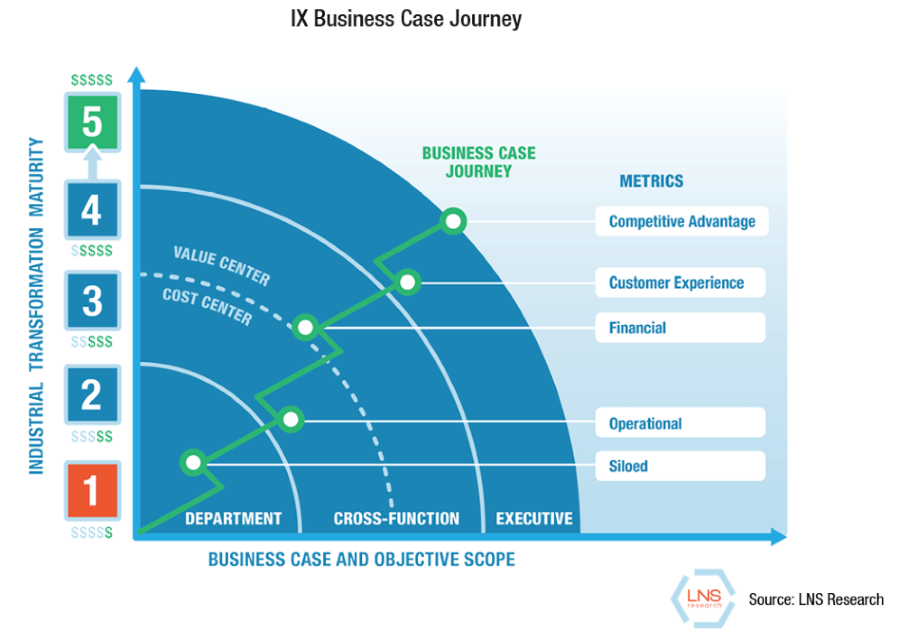
\includegraphics[width=0.75\textwidth]{assets/value_center.png}
\caption{Visualisasi Pergeseran Paradigma: Dari \textit{Cost Center} Menuju \textit{Value Center}}
\end{figure}

Tiga prinsip fundamental yang mendasari evaluasi prosedur perlu dipahami oleh Manajemen Atas:

\begin{figure}[H]
\centering
\resizebox{0.85\textwidth}{!}{%
\begin{tikzpicture}[scale=1.0]
    % === Stage 1: Value-Added Focus ===
    \node[rectangle, rounded corners=4pt, draw=plnblue, fill=plnblue!8, minimum width=3cm, minimum height=1.6cm, align=center] (b1) at (0,0) {};
    \node[font=\scriptsize\bfseries, text=plnblue] at (0,0.5) {Value-Added Focus};
    \node[font=\tiny, text=gray!80!black] at (0,0.2) {Hapus yang tidak perlu};
    \node[fill=red!25, draw=red, minimum size=0.25cm, inner sep=0pt] at (-0.6,-0.2) {};
    \draw[red, very thin] (-0.7,-0.1) -- (-0.5,-0.3); \draw[red, very thin] (-0.7,-0.3) -- (-0.5,-0.1);
    \node[fill=plngreen!25, draw=plngreen, minimum size=0.25cm, inner sep=0pt] at (0,-0.2) {};
    \node[fill=red!25, draw=red, minimum size=0.25cm, inner sep=0pt] at (0.6,-0.2) {};
    \draw[red, very thin] (0.5,-0.1) -- (0.7,-0.3); \draw[red, very thin] (0.5,-0.3) -- (0.7,-0.1);
    
    \draw[-{Stealth[length=5pt]}, thick, gray!50] (1.6,0) -- (2.2,0);
    
    % === Stage 2: Single Source of Truth ===
    \node[rectangle, rounded corners=4pt, draw=plncyan, fill=plncyan!8, minimum width=3cm, minimum height=1.6cm, align=center] (b2) at (4,0) {};
    \node[font=\scriptsize\bfseries, text=plncyan] at (4,0.5) {Single Source of Truth};
    \node[font=\tiny, text=gray!80!black] at (4,0.2) {Input 1×, pakai banyak};
    \fill[plncyan!50] (4,-0.15) circle (0.1cm);
    \draw[plncyan, thin] (4,-0.15) -- (3.65,-0.35); \draw[plncyan, thin] (4,-0.15) -- (4,-0.4); \draw[plncyan, thin] (4,-0.15) -- (4.35,-0.35);
    \fill[plncyan!30] (3.65,-0.35) circle (0.05cm); \fill[plncyan!30] (4,-0.4) circle (0.05cm); \fill[plncyan!30] (4.35,-0.35) circle (0.05cm);
    
    \draw[-{Stealth[length=5pt]}, thick, gray!50] (5.6,0) -- (6.2,0);
    
    % === Stage 3: Rule-Based Routing ===
    \node[rectangle, rounded corners=4pt, draw=plnorange, fill=plnorange!8, minimum width=3cm, minimum height=1.6cm, align=center] (b3) at (8,0) {};
    \node[font=\scriptsize\bfseries, text=plnorange] at (8,0.5) {Rule-Based Routing};
    \node[font=\tiny, text=gray!80!black] at (8,0.2) {Otomatis berdasarkan aturan};
    \node[diamond, fill=plnorange!25, draw=plnorange, aspect=1, minimum size=0.35cm, inner sep=0pt] at (8,-0.15) {};
    \draw[-{Stealth[length=4pt]}, plngreen, thin] (8.2,-0.1) -- ++(0.25,0.12);
    \draw[-{Stealth[length=4pt]}, red, thin] (8.2,-0.2) -- ++(0.25,-0.12);
\end{tikzpicture}
}
\caption{Tiga Pilar Strategis Optimalisasi Prosedur}
\end{figure}

\textit{\textit{value-added} Analysis} adalah prinsip yang menyatakan bahwa setiap langkah dalam alur kerja harus diuji apakah benar-benar menambah nilai bagi pelanggan (unit berikutnya, auditor, atau regulator) atau sekadar \textit{waste}. Dalam konteks PLN, langkah seperti mencetak dokumen hanya untuk ditandatangani, mengirim berkas fisik antar-lantai, atau mengetik ulang data yang sudah tersedia di SAP merupakan \textit{\textit{non-\textit{value-added}} activities} yang harus dieliminasi.

\textit{Single Source of Truth} memastikan bahwa data cukup diinput satu kali di sistem sumber operasional (misal: SAP-PM, E-Procurement, SCADA) dan berpindah secara otomatis beserta metadata-nya ke repositori kearsipan tanpa intervensi rekam ulang secara manual.

\textit{Rule-Based Routing} merujuk pada pendelegasian pergerakan dokumen kepada sistem. Dokumen tidak lagi diedarkan secara manual, melainkan dikirim otomatis ke Pejabat Berwenang sesuai dengan parameter matriks persetujuan (SLA) yang ditanamkan dalam aplikasi.

\subsection*{Dampak Inefisiensi: \textit{Friction Points} pada Tata Kelola Konvensional}

Ketika ketiga pilar strategis tersebut diabaikan, organisasi akan terus berada dalam siklus administrasi konvensional yang memicu \textit{waste}. Ketidakmampuan dalam merancang tata kelola kearsipan yang terintegrasi ini seringkali berujung pada pola inefisiensi sistemik, yang dapat divisualisasikan melalui dua skenario \textit{friction points} berikut:


\begin{figure}[H]
\centering
\begin{minipage}{0.95\textwidth}
\begin{tcolorbox}[
    colback=white, colframe=plnblue!40,
    boxrule=0.6pt, arc=3pt, left=3pt, right=3pt, top=2pt, bottom=2pt,
    title={\footnotesize\bfseries \color{plnblue}Skenario 1: Digital $\rightarrow$ Analog $\rightarrow$ Digital},
    fonttitle=\bfseries, coltitle=plnblue,
    attach boxed title to top left={yshift=-2.5mm, xshift=4mm},
    boxed title style={colback=white, colframe=white, boxrule=0pt}
]
\centering
\resizebox{0.95\textwidth}{!}{%
\begin{tikzpicture}[node distance=1.0cm]
\node[draw, fill=plnblue!10, text width=2.0cm, align=center, font=\tiny, rounded corners=2pt] (s1) {Penciptaan\\(Sistem A)};
\node[draw, red, fill=red!10, right=of s1, text width=2.0cm, align=center, font=\tiny, rounded corners=2pt] (f1) {CETAK FISIK\\(Friction 1)};
\node[draw, red, fill=red!10, right=of f1, text width=2.0cm, align=center, font=\tiny, rounded corners=2pt] (f2) {TTD MANUAL\\(Friction 2)};
\node[draw, red, fill=red!10, right=of f2, text width=2.0cm, align=center, font=\tiny, rounded corners=2pt] (f3) {SCAN \& UPLOAD\\(Friction 3)};
\node[draw, fill=plnblue!10, right=of f3, text width=2.0cm, align=center, font=\tiny, rounded corners=2pt] (s2) {Penyimpanan\\(Sistem B)};
\draw[->, thick] (s1) -- (f1); \draw[->, thick] (f1) -- (f2); \draw[->, thick] (f2) -- (f3); \draw[->, thick] (f3) -- (s2);
\end{tikzpicture}%
}
\end{tcolorbox}
\vspace{0.2cm}
\begin{tcolorbox}[
    colback=white, colframe=plnorange!50,
    boxrule=0.6pt, arc=3pt, left=3pt, right=3pt, top=2pt, bottom=2pt,
    title={\footnotesize\bfseries \color{plnorange}Skenario 2: Fisik Sejak Awal},
    fonttitle=\bfseries, coltitle=plnorange,
    attach boxed title to top left={yshift=-2.5mm, xshift=4mm},
    boxed title style={colback=white, colframe=white, boxrule=0pt}
]
\centering
\resizebox{0.75\textwidth}{!}{%
\begin{tikzpicture}[node distance=1.0cm]
\node[draw, red, fill=red!10, text width=2.2cm, align=center, font=\tiny, rounded corners=2pt] (p1) {PENCIPTAAN FISIK\\(Formulir Manual)};
\node[draw, red, fill=red!10, right=of p1, text width=2.2cm, align=center, font=\tiny, rounded corners=2pt] (p2) {DISTRIBUSI FISIK\\(Kurir/Pos Internal)};
\node[draw, red, fill=red!10, right=of p2, text width=2.2cm, align=center, font=\tiny, rounded corners=2pt] (p3) {PENYIMPANAN FISIK\\(Lemari Arsip)};
\node[draw, red, fill=red!10, right=of p3, text width=2.2cm, align=center, font=\tiny, rounded corners=2pt] (p4) {DIGITALISASI\\(Scan saat butuh)};
\draw[->, thick] (p1) -- (p2); \draw[->, thick] (p2) -- (p3); \draw[->, thick] (p3) -- (p4);
\end{tikzpicture}%
}
\end{tcolorbox}
\end{minipage}
\caption{Friction Points (Titik Inefisiensi) pada Skenario Prosedur Kearsipan As-Is}
\end{figure}

Pertimbangkan skenario berikut: jika proses persetujuan Berita Acara Serah Terima (BAST) pembangkit memerlukan waktu 5 hari karena harus melewati antrean cetak, kurir, dan tanda tangan basah, maka pembayaran kepada vendor tertunda, proyek pembangkit terhambat, dan PLN menghadapi risiko ganda: (1) kerugian finansial akibat keterlambatan operasional, serta (2) sanksi regulasi jika audit trail tidak lengkap. Dalam perspektif GCG, kegagalan mengoptimasi prosedur secara langsung memengaruhi penilaian tata kelola perusahaan -- termasuk dalam parameter TARIF yang menjadi tolok ukur kinerja BUMN.

\subsection*{Solusi Paradigma: Model \textit{Records Continuum}}
Sebagai solusi dari inefisiensi pada Skenario 1 dan 2, Manajemen Atas harus mengadopsi kerangka kerja \textbf{\textit{Records Continuum Model}} (ISO 15489). Berbeda dengan siklus hidup tradisional (\textit{Life Cycle}) yang memutus umur dokumen menjadi fase-fase terpisah (aktif, inaktif, musnah), \textit{Continuum Model} menegaskan bahwa arsip digital adalah satu aliran data berkesinambungan sejak ia dikonsepkan di aplikasi operasional.

\begin{figure}[H]
\centering
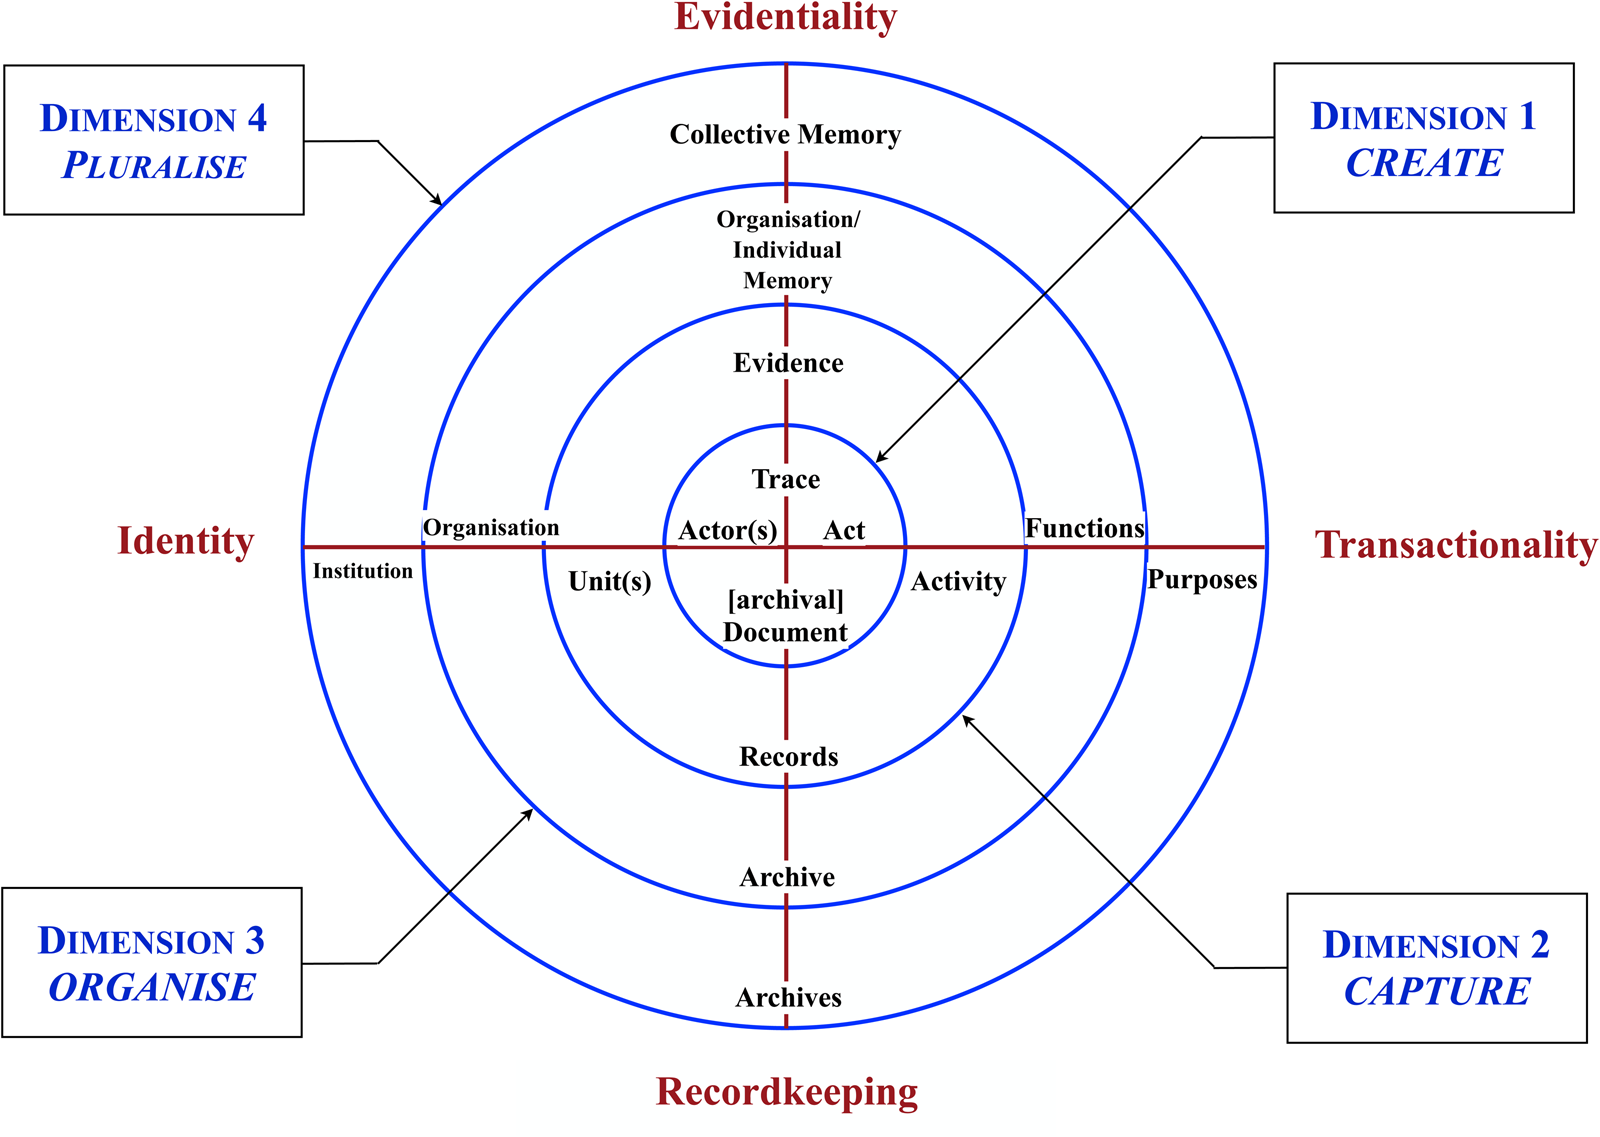
\includegraphics[width=0.75\textwidth]{assets/rc3.png}
\caption{Model Records Continuum: Arsip sebagai Aliran Data yang Tak Terputus (Sumber: Upward, 1996)}
\end{figure}

Dimensi kontinuitas ini mencakup:
\begin{itemize}[leftmargin=*]
    \item \textbf{Create:} Transaksi awal terekam otomatis saat kejadian (contoh: BAST/SPK diterbitkan).
    \item \textbf{Capture:} Sistem mengunci validasi dan metadata untuk integritas hukum.
    \item \textbf{Organize:} Klasifikasi otonom yang langsung mengatur tata kelola organisasi.
    \item \textbf{Pluralize:} Akses korporat lintas-direktorat untuk audit dan kepatuhan.
\end{itemize}

\needspace{4\baselineskip}

\needspace{4\baselineskip}

\section{Teknik Pencarian Fakta untuk Manajemen Atas}

Untuk beralih dari inefisiensi administrasi konvensional menuju idealita tata kelola \textit{Records Continuum}, Manajemen Atas harus terlebih dahulu memetakan presisi akar masalah di unit kerjanya. Proses pemetaan ini menuntut ketersediaan data faktual dari lapangan, bukan sekadar opini atau asumsi di atas kertas. 

Bagi Manajemen Atas, pengumpulan fakta operasional ini bukan berarti turun langsung melakukan audit teknis sendirian, melainkan memastikan bahwa tim pengampu kearsipan menjalankan tiga metodologi investigasi berikut dan menyajikan temuannya secara terukur:

\begin{enumerate}[leftmargin=*]
    \item Document Shadowing. Tim operasional melingkupi siklus hidup satu dokumen dari penciptaan hingga penyimpanan. Catat setiap kali dokumen berpindah tangan, berganti format, atau menunggu di meja seseorang. Manajemen Atas memvalidasi apakah sampel yang dipilih representatif dan apakah temuan waktu tunggu sudah dikorelasikan dengan volume aktual.
    \item Log Analysis. Tim IT membuka data \textit{timestamp} sistem dan bandingkan \textit{actual vs SLA}. Berapa lama seharusnya proses persetujuan versus kenyataannya? Manajemen Atas memastikan bahwa perbandingan ini tidak hanya teknis, melainkan dikaitkan dengan dampak bisnis (keterlambatan pembayaran vendor, penalti kontrak, dll).
    \item Gemba Walk. Tim manajemen turun langsung ke lapangan dan bertanya kepada staf: ``Apa yang paling membuat frustrasi?'' ``Berapa kali Anda input ulang data yang sama ke sistem berbeda?'' Manajemen Atas memastikan bahwa temuan dari Gemba Walk tidak hanya didengar, melainkan dituangkan dalam daftar perbaikan prioritas.
\end{enumerate}

\begin{figure}[H]
\centering
\resizebox{0.85\textwidth}{!}{%
\begin{tikzpicture}[scale=0.55, every node/.style={transform shape}]
    % Steps as Boxes
    % Shadowing
    \node[rectangle, rounded corners=6pt, draw=plnblue, fill=plnblue!5, minimum width=3.5cm, minimum height=2.2cm, align=center] (a) at (0,0) {};
    \node[font=\scriptsize\bfseries, text=plnblue] at (0,0.7) {Shadowing};
    \begin{scope}[shift={(0,-0.2)}]
        \draw[thick, plnblue] (-0.3,0) rectangle (0.3,0.5);
        \draw[plnblue] (-0.2,0.4) -- (0.2,0.4); \draw[plnblue] (-0.2,0.3) -- (0.2,0.3);
        \draw[plnorange, very thick] (0.3,0) circle (0.25cm);
        \draw[plnorange, very thick] (0.45,-0.15) -- (0.6,-0.3);
    \end{scope}

    % Log Analysis
    \node[rectangle, rounded corners=6pt, draw=plncyan, fill=plncyan!5, minimum width=3.5cm, minimum height=2.2cm, align=center] (b) at (4.5,2.5) {};
    \node[font=\scriptsize\bfseries, text=plncyan] at (4.5,3.2) {Log Analysis};
    \begin{scope}[shift={(4.5,2.3)}]
        \draw[->, gray] (-0.5,0) -- (0.5,0); \draw[->, gray] (-0.5,0) -- (-0.5,0.7);
        \draw[thick, plncyan] (-0.5,0.1) -- (-0.2,0.5) -- (0.1,0.3) -- (0.4,0.6);
    \end{scope}

    % Gemba Walk
    \node[rectangle, rounded corners=6pt, draw=plnorange, fill=plnorange!5, minimum width=3.5cm, minimum height=2.2cm, align=center] (c) at (9,0) {};
    \node[font=\scriptsize\bfseries, text=plnorange] at (9,0.7) {Gemba Walk};
    \begin{scope}[shift={(9,-0.2)}]
        \draw[thick, plnorange] (0,0.4) circle (0.15cm);
        \draw[thick, plnorange] (0,0.25) -- (0,-0.1);
        \draw[thick, plnorange] (-0.2,0.1) -- (0.2,0.1);
        \draw[plngreen, very thick] (0.4,0) -- (0.5,-0.1) -- (0.7,0.2);
    \end{scope}

    % Arrows
    \draw[-{Stealth[length=8pt]}, line width=1.5pt, gray!30] (1.8,0.5) .. controls (2.5,1.5) .. (3.2,2.0);
    \draw[-{Stealth[length=8pt]}, line width=1.5pt, gray!30] (5.8,2.0) .. controls (6.5,1.5) .. (7.2,0.5);
\end{tikzpicture}%
}
\caption{Visualisasi Proses Diagnosa Lapangan: Shadowing, Log Analysis, dan Gemba Walk}
\end{figure}




\needspace{4\baselineskip}

\section{Kerangka Diagnosa 7 Domain Terintegrasi}

Data mentah dan temuan yang berhasil dikumpulkan melalui \textit{Shadowing}, \textit{Log Analysis}, dan \textit{Gemba Walk} pada akhirnya harus dikuantifikasi agar dapat dijadikan dasar keputusan bisnis. Untuk itu, seluruh temuan lapangan tersebut wajib dipetakan dan diskor ke dalam kerangka evaluasi yang komprehensif.

Ketujuh domain berikut adalah instrumen standar untuk menilai tingkat kematangan tata kelola arsip PLN: mulai dari dimensi kebijakan hingga arsitektur teknologi. Karena disusun berdasarkan sintesis regulasi nasional dan standar global (ISO 15489, ANRI), hasil evaluasi pada domain ini sah untuk dijadikan dasar persetujuan anggaran dan prioritas alokasi sumber daya.
Evaluasi dilakukan dengan skor 1--5 pada tujuh domain berikut untuk menentukan prioritas optimasi. Domain ini bukan adopsi harfiah dari satu standar tunggal, melainkan hasil sintesis terstruktur dari standar kearsipan dan keamanan global (ISO, NIST, PARBICA) serta regulasi tata kelola nasional dan prinsip GCG BUMN.

\begingroup
\small
\begin{xltabular}{\textwidth}{@{} l X c @{}}
\caption{Kerangka Diagnosa 7 Domain Terintegrasi}\\
\toprule
\textbf{Domain} & \textbf{Pertanyaan Kunci} & \textbf{Skor (1--5)} \\
\midrule
\endfirsthead

\multicolumn{3}{@{}l}{\small\textit{Lanjutan Tabel \thetable}}\\
\toprule
\textbf{Domain} & \textbf{Pertanyaan Kunci} & \textbf{Skor (1--5)} \\
\midrule
\endhead

\bottomrule
\endfoot

\rowcolor{rowalt}
1. Kebijakan & Apakah ada mandat penciptaan arsip di titik transaksi? Apakah kebijakan kearsipan terintegrasi dengan kebijakan korporasi? & $\square$ \\
2. Tata Kelola & Apakah peran dan akuntabilitas (RACI) sudah jelas? Apakah ada pemisahan fungsi antara pencipta, pengelola, dan pengguna arsip? & $\square$ \\
\rowcolor{rowalt}
3. SDM & Apakah ada KPI khusus terkait akurasi pengarsipan? Apakah staf dilatih untuk alur kerja terintegrasi? & $\square$ \\
4. Interoperabilitas & Apakah sistem mampu melakukan tarik data otomatis antar-platform (SAP, E-Office, E-Proc)? & $\square$ \\
\rowcolor{rowalt}
5. Proses Bisnis & Apakah ada duplikasi input (ketik ulang) data? Apakah ada \textit{shadow systems} (proses manual di samping sistem digital)? & $\square$ \\
6. Keamanan & Apakah audit trail bersifat \textit{immutable}? Apakah ada kontrol akses berbasis peran (RBAC)? & $\square$ \\
\rowcolor{rowalt}
7. Preservasi & Apakah format digital memenuhi standar jangka panjang (PDF/A)? Apakah strategi backup memenuhi 3-2-1? & $\square$ \\
\bottomrule
\end{xltabular}
\endgroup

Interpretasi Skor:
\begin{itemize}[leftmargin=*]
    \item $\leq$ 2 (Belum Siap): Intervensi kebijakan/desain ulang alur kerja segera. Prioritas utama.
    \item 3 (Siap Parsial): Dapat dioptimalkan melalui pemicu digital, SLA, dan exception handling.
    \item $\geq$ 4 (Siap Integrasi): Layak menjadi \textit{pilot project} alur kerja terintegrasi dan SOP digital.
\end{itemize}

\begin{plnbox}[Panduan Pemanfaatan Diagnosa untuk Keputusan Manajemen]
Gunakan hasil skoring 7 Domain sebagai dasar tiga keputusan eksekutif: (1) keputusan risiko -- domain mana yang paling rentan menimbulkan temuan audit; (2) keputusan investasi -- area mana yang perlu diprioritaskan untuk otomasi dan integrasi; dan (3) keputusan organisasi -- unit mana yang memerlukan penguatan SDM atau restrukturisasi tanggung jawab. Jangan mengesahkan rencana transformasi tanpa data diagnosa yang akurat.
\end{plnbox}

\begin{figure}[H]
\centering
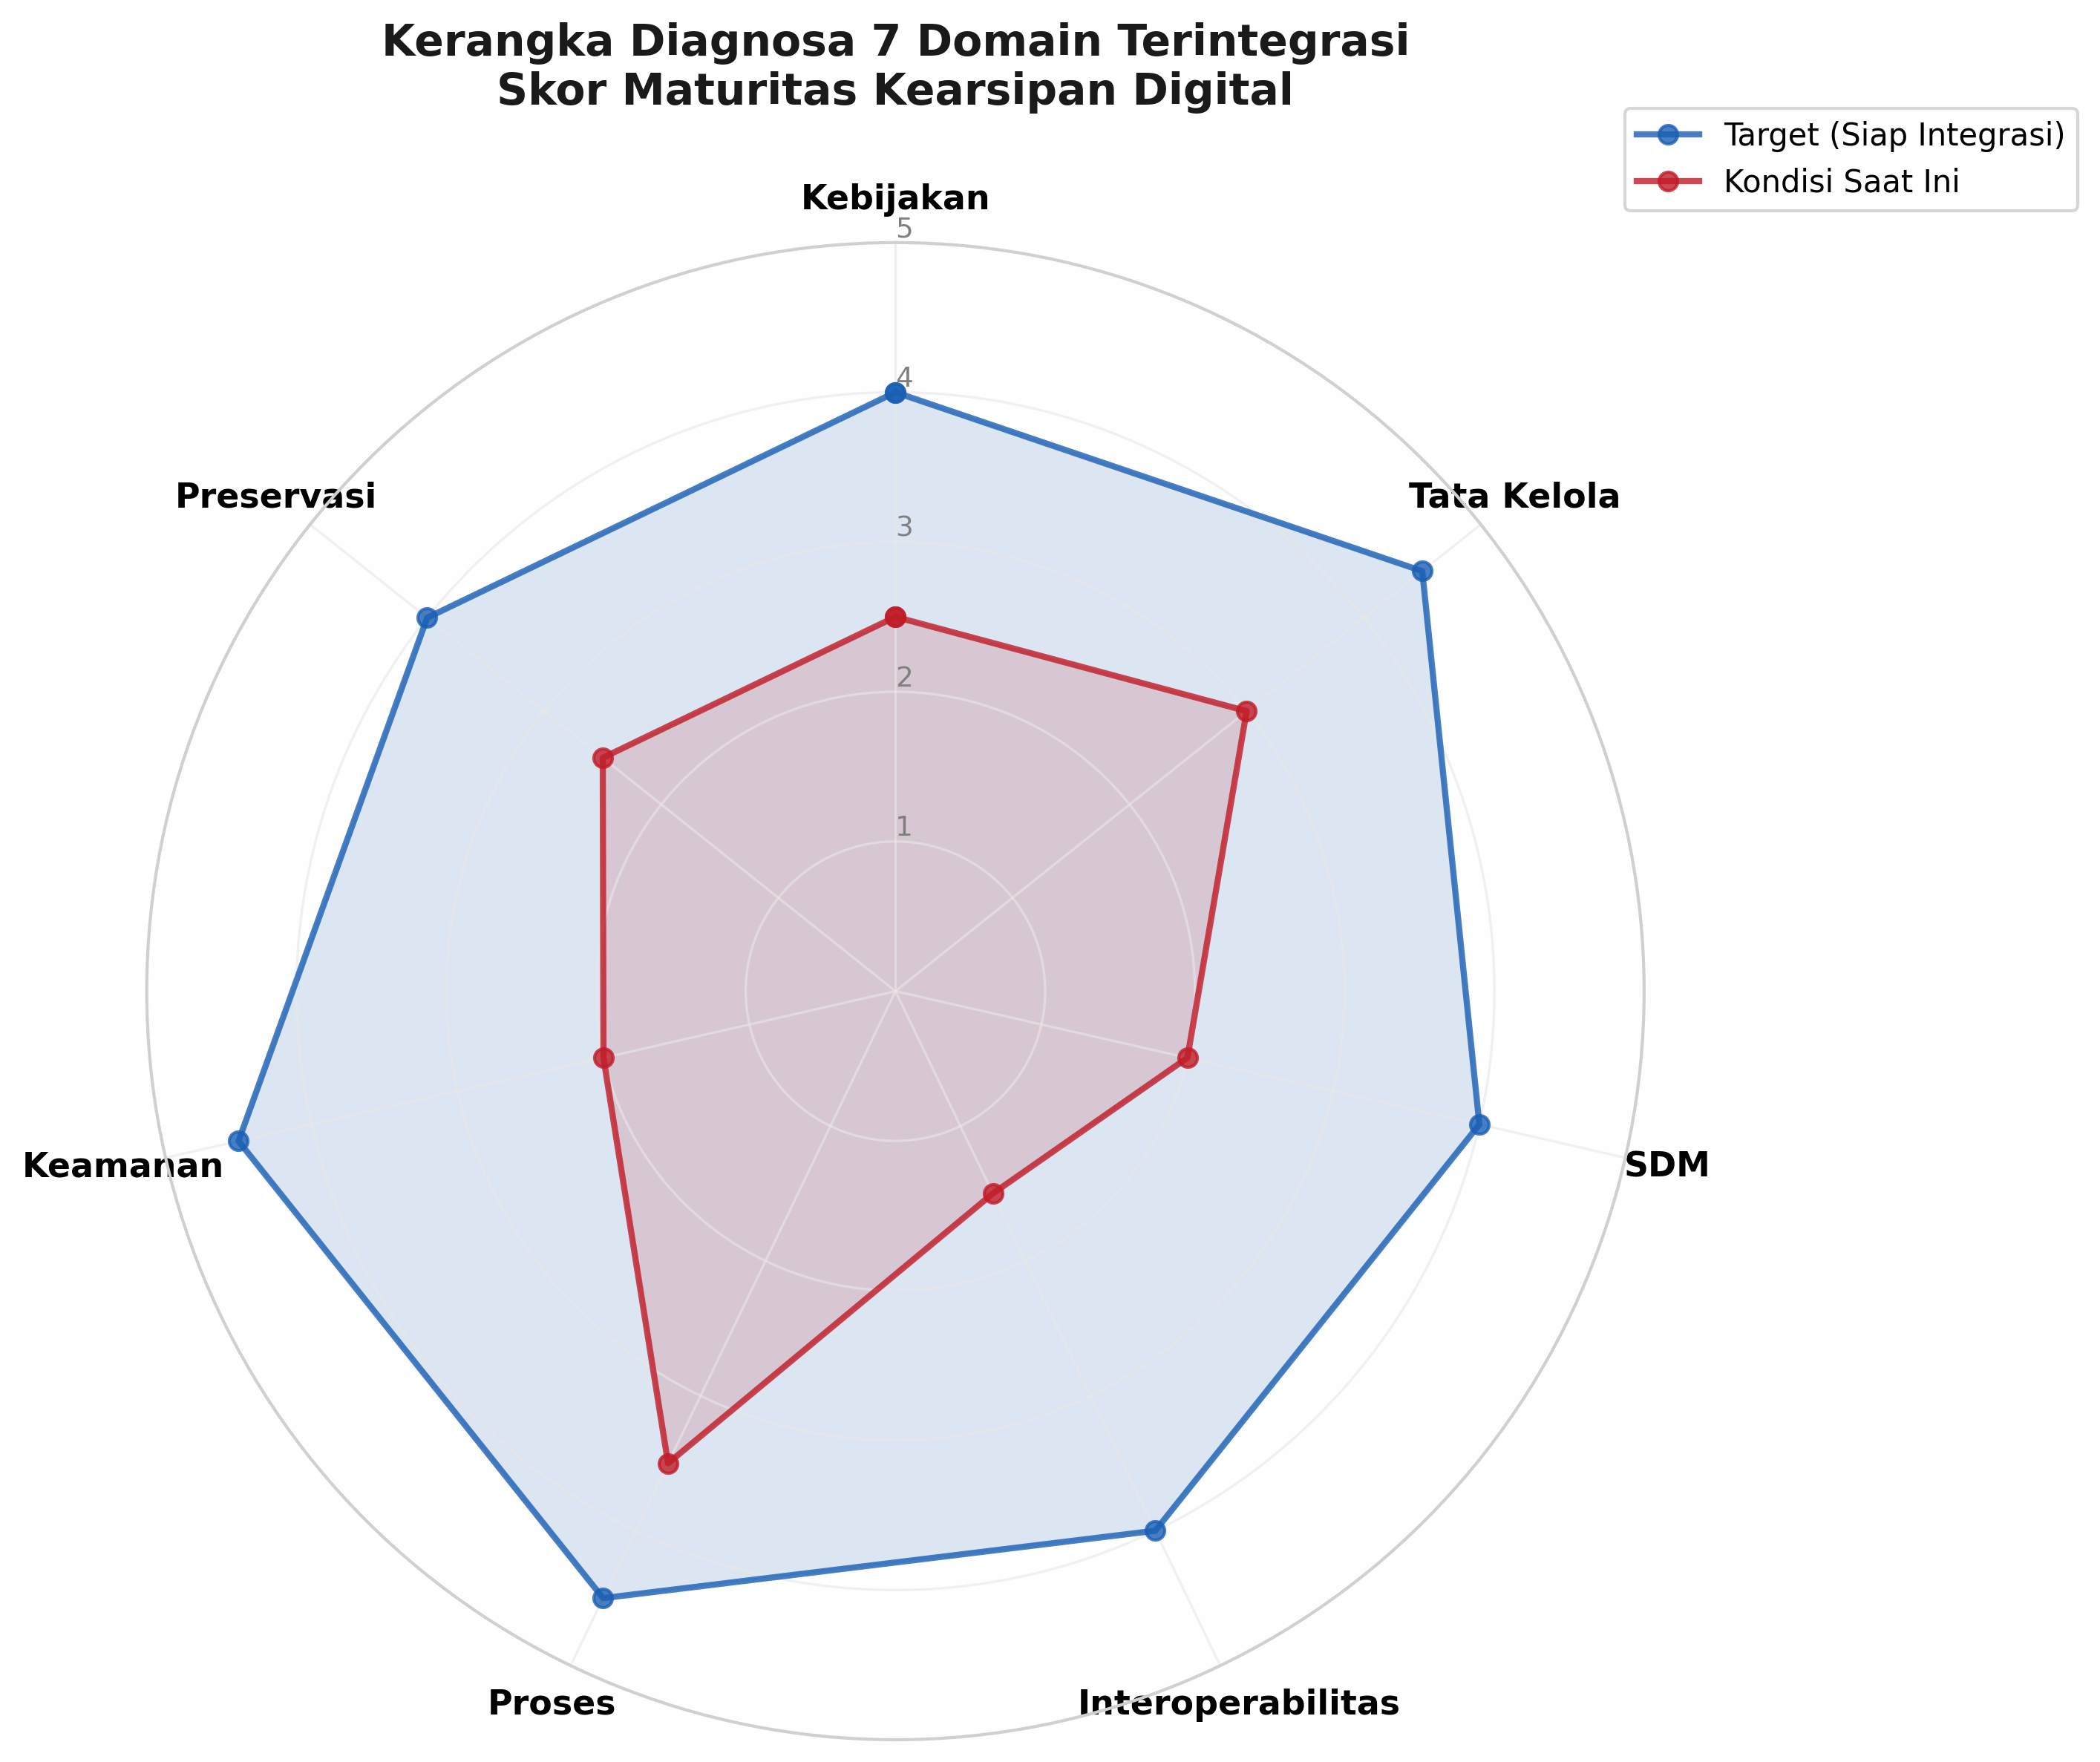
\includegraphics[width=0.85\textwidth]{assets/diagram_7domain.png}
\caption{Radar Chart Maturitas: Perbandingan Skor 7 Domain (Kondisi Saat Ini vs Target Siap Integrasi)}
\end{figure}

\begin{warnbox}[Peringatan: Data Asumsi vs Faktual]
Angka kerugian yang digunakan dalam simulasi modul ini (misalnya Rp 1,04 Miliar/tahun) adalah ilustrasi pemodelan pedagogis. Di workshop, Bapak/Ibu wajib mengganti angka-asumsi ini dengan data faktual unit masing-masing agar justifikasi bisnis akuntabel di depan komite investasi.
\end{warnbox}

\needspace{4\baselineskip}

\section{Langkah-Langkah Evaluasi Prosedur}

Hasil skoring dari 7 Domain (seperti tergambar pada Radar Chart) telah mendokumentasikan posisi maturitas (\textit{maturity level}) kearsipan organisasi saat ini secara objektif. Untuk meramu hasil pemetaan statis tersebut menjadi rencana perbaikan yang berdampak nyata, Manajemen Atas perlu memandu tim unitnya melalui lima tahapan evaluasi prosedural yang progresif berikut:

\begin{enumerate}[leftmargin=*]
    \item Pilih Proses Prioritas. Manajemen Atas menetapkan 1--2 proses kearsipan dengan volume tinggi atau risiko tinggi sebagai pilot evaluasi. Contoh: BAST E-Procurement, SPK Pemeliharaan GI, atau Laporan Keuangan Bulanan.
    \item Terapkan 7 Domain. Tim lintas fungsi (Kearsipan, IT, Operasional) melakukan skoring pada 7 Domain. Manajemen Atas memvalidasi kelengkapan data dan kejujuran skoring -- jangan biarkan unit melakukan \textit{self-rating} yang terlalu optimis.
    \item Identifikasi \textit{Waste Terbesar.} Fokus pada 3 jenis \textit{waste} utama: \textit{Overprocessing} (mencetak hanya untuk tanda tangan), \textit{Waiting} (dokumen tertahan di antrean persetujuan), dan \textit{Defect} (kesalahan metadata yang memerlukan revisi).
    \item Kuantifikasi Dampak Bisnis. Ubah temuan waste menjadi angka: berapa jam terbuang per tahun, berapa biaya revisi, berapa risiko sanksi jika audit trail tidak lengkap. Tanpa kuantifikasi, temuan diagnosa tidak akan mendapatkan perhatian komite investasi.
    \item Tetapkan Prioritas Intervensi. Manajemen Atas menyetujui daftar area optimasi yang diurutkan berdasarkan dampak bisnis vs biaya intervensi. Prioritaskan \textit{quick wins} yang dapat menunjukkan hasil dalam 30--60 hari.
\end{enumerate}

Pertanyaan kunci untuk Manajemen Atas: ``Apakah kita tahu persis berapa lama waktu siklus proses arsip vital di unit ini, dan berapa persen dari waktu itu adalah \textit{waste} yang bisa dieliminasi?''

\begin{plnbox}[Ringkasan untuk Manajemen Atas -- Bab 1]
Diagnosa adalah tahap awal dan penentu optimalisasi: tanpa data akurat tentang apa yang salah, solusi yang dirancang akan tidak tepat sasaran. Tiga pesan kunci yang harus dibawa Manajemen Atas dari bab ini: (1) diagnosa harus berbasis 7 Domain yang mencakup kebijakan, tata kelola, SDM, interoperabilitas, proses, keamanan, dan preservasi; (2) data faktual lebih bernilai daripada asumsi -- minta tim menyajikan bukti waktu tunggu, volume revisi, dan frekuensi kehilangan; dan (3) prioritas intervensi harus didasarkan pada dampak bisnis, bukan kemudahan teknis implementasi.
\end{plnbox}

\needspace{4\baselineskip}

\section{Aktivitas Workshop (30 Menit)}
\textit{(Catatan: Gunakan \textbf{Lampiran A: Matriks Identifikasi Area Optimasi} pada Lembar Kerja untuk aktivitas ini.)}
\begin{enumerate}[leftmargin=*]
    \item Pilih 1 proses kearsipan di unit Anda dan lakukan Document Shadowing ringkas (catat setiap langkah, waktu, dan format).
    \item Skor 7 Domain untuk proses tersebut dan identifikasi domain paling lemah.
    \item Kuantifikasi \textit{waste} dalam satuan jam/tahun dan biaya kesempatan (opportunity cost).
\end{enumerate}

\begin{outputbox}
Portofolio 1 (Fase 1: Diagnosa): Matriks Identifikasi Area Optimasi + Skoring 7 Domain. Dinilai berdasarkan kemampuan peserta mengevaluasi prosedur \textit{as-is} secara sistematis, kejelasan temuan \textit{waste}, kuantifikasi dampak bisnis, dan prioritas intervensi yang masuk akal.
\end{outputbox}


% ============================================================
\chapter{Desain: Perancangan Alur Kerja Terintegrasi (\textit{to-be})}
(Kriteria Penilaian 4.3.2 -- Target Kompetensi 2)
% ============================================================

Bab ini mendukung pencapaian Fase 2: Desain Alur Kerja -- peserta mampu merancang alur kerja terintegrasi (\textit{to-be}) berbasis BPMN 2.0 dengan pemicu otomatis dan pola integrasi. 

Setelah memetakan inefisiensi sistemik pada Fase Diagnosa (Bab 1), Manajemen Atas membutuhkan arsitektur operasional baru untuk mengatasi inefisiensi tersebut. Temuan diagnosa hanyalah identifikasi masalah; penyelesaiannya terletak pada perancangan ulang tata kelola alur kerja. Desain alur kerja (Fase 2) hadir untuk merumuskan cara kerja baru yang mengeliminasi \textit{waste} secara otomatis. Desain baru ini bukan sekadar aktivitas menggambar diagram teknis, melainkan penyusunan arsitektur hukum yang mengikat unit kerja ke dalam sebuah notasi visual standar internasional (BPMN).

\needspace{4\baselineskip}

\section{Tiga Pola Integrasi Utama PLN}
Implementasi alur kerja terintegrasi di organisasi sebesar PLN tidak berarti menjalankan seluruh proses secara otomatis dengan prioritas yang sama. Pola integrasi berikut memetakan prioritas implementasi berdasarkan dampak bisnis dan kompleksitas teknis:

\begin{plnbox}[Pola 1: Trigger-Based Auto-Capture]
Sistem operasional (ERP/SCADA) secara otomatis menarik data transaksi dan menghasilkan draf arsip beserta metadata begitu status transaksi final. \textit{Manusia tidak lagi memulai proses arsip secara manual.} Contoh: teknisi menekan ``Technical Complete'' di aplikasi operasional, dan detik itu juga draf BA Penormalan tercipta dengan metadata lengkap.

Makna bagi Manajemen Atas: Ini adalah prasyarat kepatuhan. Tanpa auto-capture, organisasi bergantung pada kesadaran dan kesempatan manusia untuk mengarsipkan -- sebuah risiko yang tidak dapat diterima untuk transaksi bernilai miliaran rupiah.
\end{plnbox}

\begin{plnbox}[Pola 2: Parallel Digital Routing]
Dokumen dikirim serentak ke multi-pejabat (misal: \textit{Asset Owner} \& \textit{Dispatcher}) untuk persetujuan paralel. Ini memangkas antrean birokrasi berjenjang secara dramatis.

Makna bagi Manajemen Atas: Pengurangan waktu siklus 60--80\% pada proses persetujuan. Namun, Manajemen Atas harus memastikan ada mekanisme penguncian \textit{read-only} dan pelacakan versi, karena persetujuan paralel tanpa kontrol akan menghasilkan kekacauan versi dokumen.
\end{plnbox}

\begin{plnbox}[Pola 3: SLA-Driven Escalation]
Jika validasi melebihi batas waktu (contoh: $>$1--16 jam sesuai jenis dokumen), sistem secara otomatis mengeskalasi ke atasan (Manajer UPT/GM). Tidak ada lagi dokumen yang tertahan di antrean persetujuan tanpa eskalasi otomatis.

Makna bagi Manajemen Atas: Ini adalah instrumen akuntabilitas. SLA dalam sistem digital bukan sekadar angka durasi target penyelesaian, melainkan kontrak akuntabilitas otomatis yang secara mekanis mencegah dokumen tertahan di meja persetujuan tanpa konsekuensi. Manajemen Atas harus menyetujui threshold SLA dan menerima notifikasi eskalasi secara aktif.
\end{plnbox}

Untuk merealisasikan ketiga pola alur kerja (logikal) di atas, PLN membutuhkan infrastruktur arsitektur pertukaran data yang tangguh antar-sistem (seperti integrasi SAP, E-Procurement, dan E-Office). Gambar berikut mengilustrasikan relevansi tersebut melalui \textbf{Tiga Pola Arsitektur Integrasi Sistem}. Pendekatan \textit{Hybrid} (kombinasi Point-to-Point dan Middleware/Hub) menjadi rekomendasi utama karena paling andal dalam mengakomodasi kompleksitas \textit{trigger} otomatis, \textit{routing} paralel, dan eskalasi SLA pada volume transaksi berskala besar.

\begin{figure}[H]
\centering
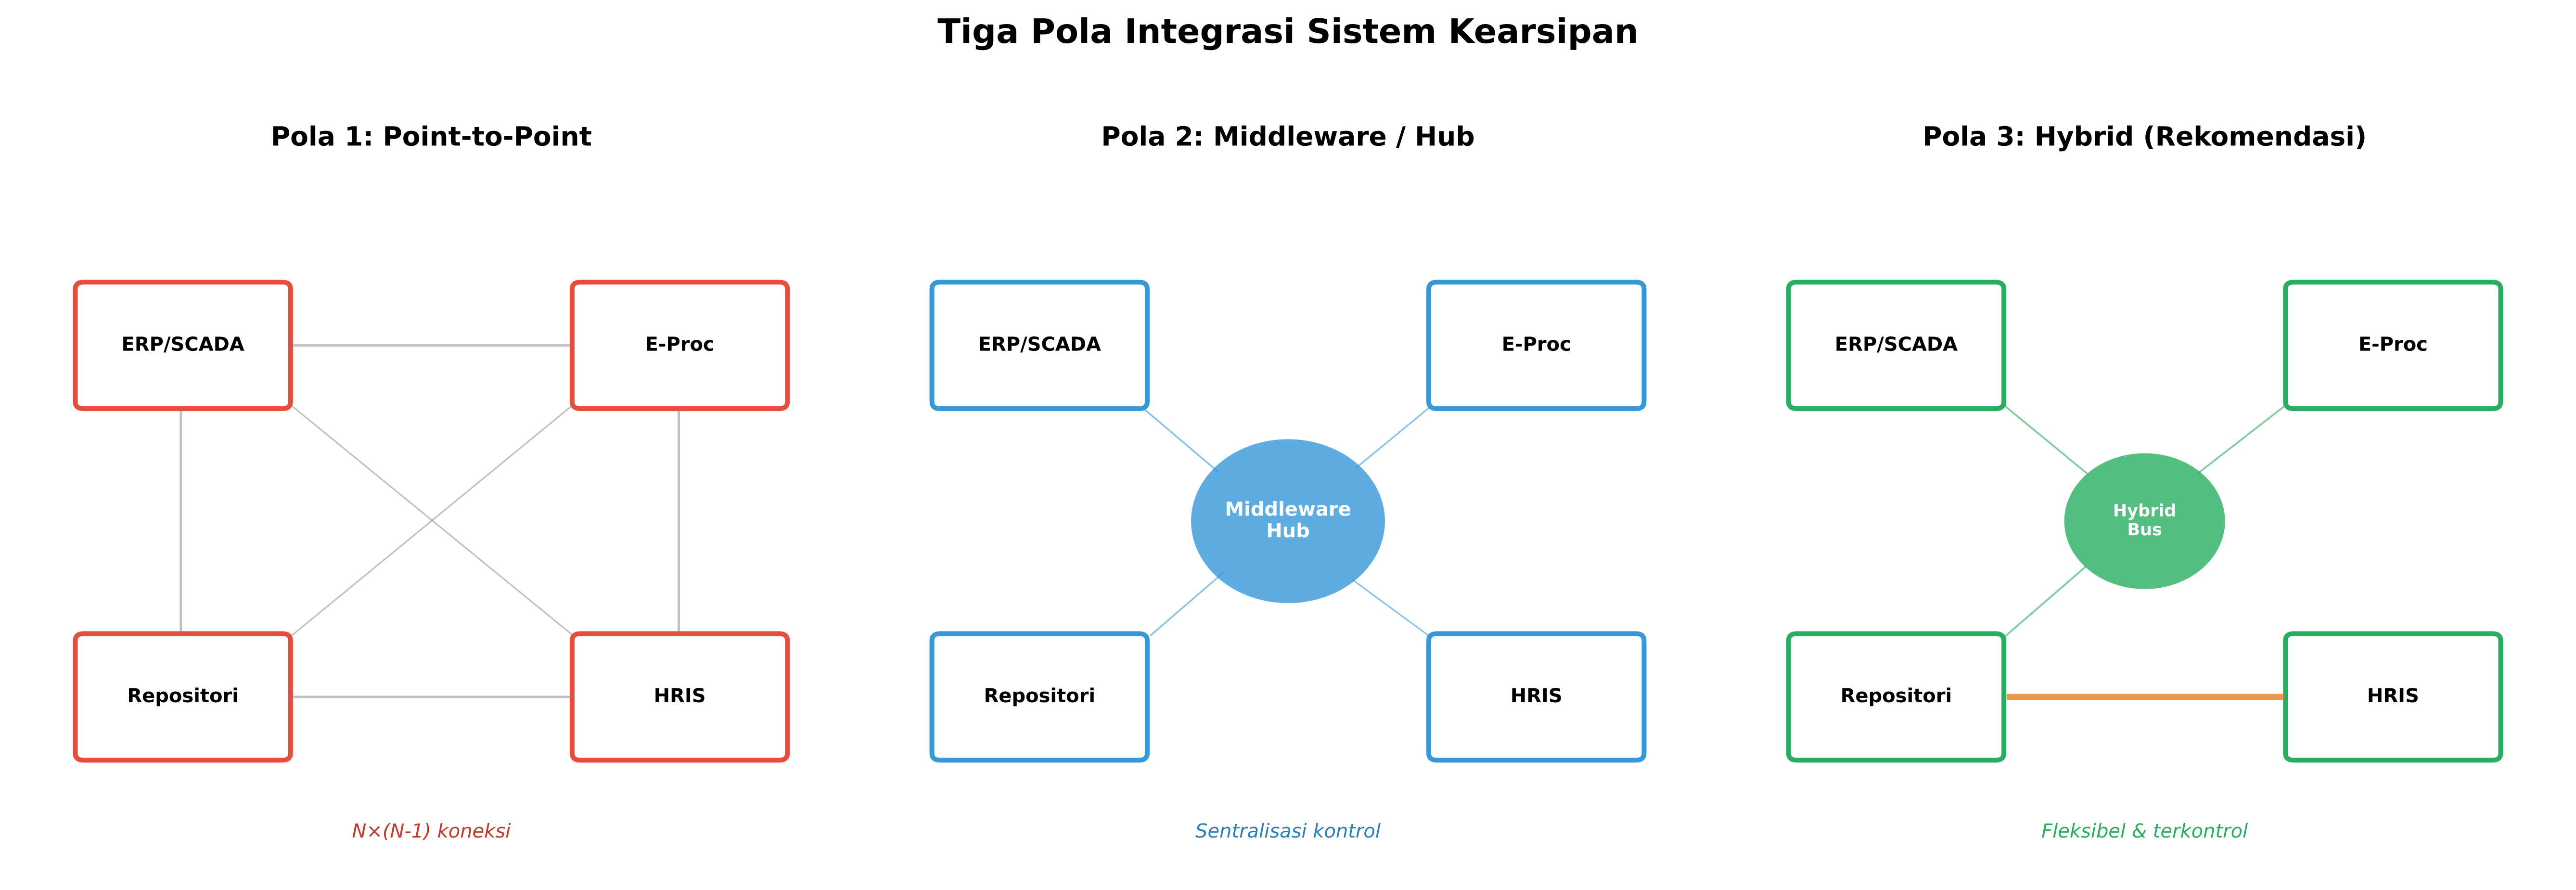
\includegraphics[width=0.95\textwidth]{assets/diagram_pola_integrasi.png}
\caption{Tiga Pola Arsitektur Integrasi Sistem: Point-to-Point, Middleware/Hub, dan Hybrid (Rekomendasi)}
\end{figure}

\needspace{4\baselineskip}

\section{Notasi BPMN 2.0 untuk Eksekutif}

Bagi Manajemen Atas, pemahaman terhadap notasi BPMN bukan tentang keahlian menggambar diagram, melainkan kemampuan membaca rancangan arsitektur proses bisnis untuk memastikan bahwa setiap langkah penting---termasuk persetujuan, pengamanan, dan audit trail---tidak terlewat dalam desain sistem. Bagian ini menyederhanakan BPMN ke level yang dapat diverifikasi dalam rapat koordinasi 15 menit.
\textit{Business Process Model and Notation (BPMN) 2.0} adalah bahasa visual standar internasional (ISO/IEC 19510)\footnote{ISO/IEC 19510:2013; lihat Daftar Pustaka [7].} untuk memetakan alur kerja. Manajemen Atas wajib bisa membaca, memvalidasi, dan mengesahkan diagram ini, karena BPMN adalah rancangan arsitektur hukum proses.

\begingroup
\small
\begin{xltabular}{\textwidth}{@{} c X X @{}}
\caption{Simbol Dasar BPMN 2.0 untuk Manajemen}\\
\toprule
\textbf{Simbol} & \textbf{Nama} & \textbf{Fungsi dalam Konteks Kearsipan} \\
\midrule
\endfirsthead

\multicolumn{3}{@{}l}{\small\textit{Lanjutan Tabel \thetable}}\\
\toprule
\textbf{Simbol} & \textbf{Nama} & \textbf{Fungsi dalam Konteks Kearsipan} \\
\midrule
\endhead

\bottomrule
\endfoot

\textbullet & Start Event & Pemicu alur (contoh: \texttt{SPK\_Selesai}, \texttt{Kontrak\_Diunggah}) \\
$\square$ & Task & Aktivitas bisnis (contoh: \texttt{Cek Kelengkapan Metadata}) \\
$\Diamond$ ($\times$) & Gateway (Exclusive) & Keputusan bercabang (\textit{Jika Disetujui / Jika Direvisi}) \\
$\rightarrow$ & Sequence Flow & Urutan tugas dalam satu sistem/unit \\
$\cdots \rightarrow$ & Message Flow & Komunikasi antar-sistem (contoh: API dari ERP ke E-Office) \\
$\blacksquare$ & End Event & Penyelesaian alur (contoh: \texttt{Arsip\_Otentik\_Disimpan}) \\
\bottomrule
\end{xltabular}
\endgroup

Mengapa Menggunakan BPMN 2.0?
\begin{itemize}[leftmargin=*]
    \item Bahasa Universal: Menyatukan komunikasi antara analis bisnis, kebijakan kearsipan, dan pengembang IT.
    \item Presisi Kepemilikan: Melalui penggunaan \textit{Pools} (lingkup unit/sistem) \& \textit{Lanes} (peran jabatan), tanggung jawab persetujuan di setiap tahapan terlihat sangat jelas.
    \item Kesiapan Otomasi: Skema logika visual BPMN dapat dieksekusi secara langsung oleh mesin otomasi (\textit{\textit{workflow} engine}).
\end{itemize}

\begin{figure}[H]
\centering
\resizebox{0.95\textwidth}{!}{%
\begin{tikzpicture}[node distance=1.2cm and 0.8cm]
\fill[gray!5] (0.2, 2.5) rectangle (18, 0.6);
\fill[yellow!4] (0.2, 0.4) rectangle (18, -2.3);
\fill[gray!5] (0.2, -2.5) rectangle (18, -5.4);
\draw[gray!30, thick] (0.2, 0.5) -- (18, 0.5);
\draw[gray!30, thick] (0.2, -2.4) -- (18, -2.4);
\node[lanelab] at (0.4, 1.6) {Staf Cabang};
\node[lanelab] at (0.4, -1.0) {Manajer UPT};
\node[lanelab] at (0.4, -4.0) {Kearsipan};
\node[startstyle] at (1.5, 1.6) (s1) {Start};
\node[manual, right=of s1] (m1) {Cetak\\Kontrak\\Rangkap 3};
\node[manual, right=of m1] (m2) {Isi Form\\Pengantar};
\node[manual, right=of m2] (m3) {Kirim Kurir\\Internal};
\node[waiting] at (8.5, -1.0) (w1) {Antrian\\Meja};
\node[manual, right=of w1] (m4) {Review\\\& TTD\\Basah};
\node[gateway, right=of m4] (g1) {$\times$};
\node[manual, right=of g1] (m5) {Stempel\\Basah};
\node[manual] at (12.5, -4.0) (m6) {Terima\\Fisik};
\node[manual, right=of m6] (m7) {Catat Buku\\Induk};
\node[endstyle, right=of m7] (e1) {End};
\draw[arr] (s1) -- (m1); \draw[arr] (m1) -- (m2); \draw[arr] (m2) -- (m3);
\draw[arr] (m3.south) -- ++(0,-0.4) -| (w1.north);
\draw[arr] (w1) -- (m4); \draw[arr] (m4) -- (g1);
\draw[arrno] (g1.north) -- ++(0,0.8) -| node[above, font=\tiny\itshape, text=red] {Revisi} (m2.south);
\draw[arr] (g1) -- node[above, font=\tiny\itshape] {OK} (m5);
\draw[arr] (m5.south) -- ++(0,-0.4) -| (m6.north);
\draw[arr] (m6) -- (m7); \draw[arr] (m7) -- (e1);
\node[timelbl, below=0.15cm of w1] {1--3 hari!};
\node[font=\small\bfseries, text=red!70!black] at (9, -6.5) {SIKLUS MANUAL: 3--5 HARI KERJA};
\end{tikzpicture}
}
\caption{Model BPMN Kondisi Saat Ini (AS-IS): Alur Manual dengan Waktu Siklus Panjang}
\end{figure}

\begin{figure}[H]
\centering
\resizebox{0.95\textwidth}{!}{%
\begin{tikzpicture}[node distance=1.2cm and 0.8cm]
\fill[plnblue!4] (0.2, 2.5) rectangle (18, 0.6);
\fill[plnorange!4] (0.2, 0.4) rectangle (18, -2.3);
\fill[plnblue!4] (0.2, -2.5) rectangle (18, -5.4);
\draw[plnblue!20, thick] (0.2, 0.5) -- (18, 0.5);
\draw[plnblue!20, thick] (0.2, -2.4) -- (18, -2.4);
\node[lanelab, text=plnblue!80!black] at (0.4, 1.6) {ERP / SAP};
\node[lanelab, text=plnblue!80!black] at (0.4, -1.0) {Pimpinan};
\node[lanelab, text=plnblue!80!black] at (0.4, -4.0) {Repositori};
\node[startstyle_tobe] at (1.5, 1.6) (s2) {Event};
\node[autostep, right=of s2] (a1) {Auto-Capture\\Metadata\\ERP};
\node[autostep, right=of a1] (a2) {Generate\\Draft Digital\\(PDF/A)};
\node[humanstep] at (7.5, -1.0) (h1) {Digital Review\\via E-Office};
\node[gateway_tobe, right=of h1] (g2) {$\times$};
\node[humanstep, right=of g2] (h2) {Otorisasi\\TTE};
\node[autostep] at (12.5, -4.0) (a3) {Hash-Lock\\Immutable};
\node[autostep, right=of a3] (a4) {Log Audit\\Trail};
\node[endstyle_tobe, right=of a4] (e2) {Arsip};
\draw[arr_tobe] (s2) -- (a1); \draw[arr_tobe] (a1) -- (a2);
\draw[arr_tobe] (a2.south) -- ++(0,-0.4) -| (h1.north);
\draw[arr_tobe] (h1) -- (g2);
\draw[arrno] (g2.north) -- ++(0,0.8) -| node[above, font=\tiny\itshape, text=red] {Batal} (a2.south);
\draw[arrok] (g2) -- node[above, font=\tiny\itshape] {Setuju} (h2);
\draw[arr_tobe] (h2.south) -- ++(0,-0.4) -| (a3.north);
\draw[arr_tobe] (a3) -- (a4); \draw[arr_tobe] (a4) -- (e2);
\node[timelbl_tobe, below=0.15cm of h1] {SLA: 16 Jam};
\node[font=\small\bfseries, text=green!50!black] at (9, -6.5) {SIKLUS DIGITAL: $<$ 24 JAM};
\end{tikzpicture}
}
\caption{Model BPMN Kondisi Target (TO-BE): Alur Terintegrasi dengan SLA Singkat}
\end{figure}

\needspace{4\baselineskip}

\section{Studi Kasus: Arsip BAST E-Procurement}
Berikut adalah skenario operasional nyata penerapan ketiga pola integrasi pada proses \textit{Berita Acara Serah Terima} (BAST) di sistem E-Procurement:

\begin{enumerate}[leftmargin=*]
    \item Pemicu: Vendor menekan ``Submit Pekerjaan'' di portal E-Procurement.
    \item Auto-Generate: Sistem menyusun draf BAST secara otomatis tanpa diketik manusia, menarik metadata vendor dan spesifikasi kontrak dari database.
    \item API Transfer: Draf dikirim ke Sistem E-Office (Tata Persuratan) via integrasi API dengan \textit{payload} metadata lengkap.
    \item \textit{review}: Manajer Logistik membuka E-Office, memeriksa substansi draf.
    \item Gateway: Ditolak $\rightarrow$ kembali ke vendor dengan komentar revisi. Disetujui $\rightarrow$ TTE (Tanda Tangan Elektronik Tersertifikasi).
    \item Hash-Lock: Sistem mengunci arsip BAST permanen (\textit{immutable}) dengan hash SHA-256.
    \item End: Transaksi BAST tervalidasi digital tanpa satu pun kertas dicetak.
\end{enumerate}

\begin{plnbox}[Relevansi untuk Unit Pengadaan]
Integrasi antara E-Procurement dan E-Office mengeliminasi kebutuhan staf mengetik ulang data vendor ke form BAST manual. Seluruh metadata kontrak tertarik otomatis dari portal pengadaan. Bagi Manajemen Atas, ini berarti: (1) eliminasi kesalahan input manual, (2) percepatan siklus persetujuan, dan (3) jejak audit trail yang lengkap untuk setiap transaksi.
\end{plnbox}

\needspace{4\baselineskip}

\section{Validasi Alur: Executive Tollgate}
Sebelum rancangan BPMN disahkan dan anggaran dicairkan, Manajemen Atas wajib memvalidasi rancangan dengan empat parameter kritis agar tidak terjadi kegagalan sistematis saat implementasi:

\begingroup
\small
\begin{xltabular}{\textwidth}{@{} l X @{}}
\caption{Executive Tollgate: Empat Parameter Validasi Alur \textit{to-be}}\\
\toprule
\textbf{Aspek Validasi} & \textbf{Pertanyaan Pemeriksaan} \\
\midrule
\endfirsthead

\multicolumn{2}{@{}l}{\small\textit{Lanjutan Tabel \thetable}}\\
\toprule
\textbf{Aspek Validasi} & \textbf{Pertanyaan Pemeriksaan} \\
\midrule
\endhead

\bottomrule
\endfoot

\rowcolor{rowalt}
1. Kelengkapan & Apakah setiap pemicu (\textit{trigger}) memiliki aktivitas (\textit{task}) dan peristiwa akhir (\textit{end event}) yang terdefinisi? \\
2. Konsistensi & Apakah semua gerbang keputusan (\textit{gateway}) memiliki jalur persetujuan \textit{dan} penolakan untuk mencegah proses terhenti? \\
\rowcolor{rowalt}
3. Kepatuhan & Apakah alur kerja telah sesuai dengan kerangka hukum dan standar kearsipan yang berlaku? \\
4. Fallback & Apakah tersedia prosedur mitigasi apabila terjadi kegagalan sistem (\textit{downtime}, API \textit{timeout})? \\
\bottomrule
\end{xltabular}
\endgroup

\begin{warnbox}[Peringatan Executive Tollgate]
Apabila salah satu kriteria di atas belum terpenuhi, jangan berikan persetujuan implementasi. Penundaan untuk perbaikan desain jauh lebih murah daripada kegagalan sistem di lapangan.
\end{warnbox}

\begin{plnbox}[Ringkasan untuk Manajemen Atas -- Bab 2]
Desain alur kerja adalah rancangan arsitektur operasional: tanpa validasi Manajemen Atas, sistem buatan IT bisa berujung pada pelanggaran wewenang persetujuan atau kebocoran akses. Tiga pesan kunci: (1) tiga pola integrasi (Trigger-Based, Parallel Routing, SLA Escalation) harus dipilih berdasarkan prioritas bisnis, bukan kemudahan teknis; (2) BPMN adalah bahasa universal yang mengikat semua pihak -- Manajemen Atas wajib bisa memvalidasinya; dan (3) \textit{Executive Tollgate} empat parameter harus dilewati sebelum satu rupiah pun dikeluarkan untuk implementasi.
\end{plnbox}

\needspace{4\baselineskip}

\section{Aktivitas Workshop (30 Menit)}
\textit{(Catatan: Gunakan \textbf{Lampiran B: Lembar Kerja Diagram BPMN To-Be} untuk aktivitas ini.)}
\begin{enumerate}[leftmargin=*]
    \item Pilih 1 proses dari hasil diagnosa Bab 1 dan gambar sketsa alur \textit{to-be} menggunakan notasi BPMN pada lembar kerja yang tersedia.
    \item Tentukan trigger sistem, jalur paralel (jika ada), threshold SLA, dan jalur eskalasi.
    \item Identifikasi 1 risiko potensial dan rancang mekanisme \textit{fallback}-nya.
\end{enumerate}

\begin{outputbox}
Portofolio 2 (Fase 2: Desain Alur Kerja): Diagram BPMN 2.0 \textit{to-be} + Peta Pemicu Integrasi. Dinilai berdasarkan kemampuan peserta merancang alur kerja terintegrasi, kejelasan trigger, konsistensi gateway, kepatuhan regulasi, dan mekanisme fallback.
\end{outputbox}


% ============================================================
\chapter{SOP Digital: Penyusunan SOP Terintegrasi 8 Komponen}
(Kriteria Penilaian 4.3.3 -- Target Kompetensi 3)
% ============================================================

Bab ini mendukung pencapaian Fase 3: SOP Digital -- peserta mampu menyusun SOP Digital Terintegrasi 8 Komponen yang memenuhi persyaratan regulasi secara komprehensif. 

Rancangan alur kerja BPMN pada Fase 2 telah berhasil memetakan \textit{blueprint} arsitektur otomasi. Namun, walaupun sistem tata kelola IT yang dibangun telah lengkap, diagram tersebut tidak memiliki kekuatan hukum apabila tidak dibakukan. SOP Digital hadir untuk memberikan legitimasi hukum terhadap rancangan tersebut. Ia bukan sekadar dokumen manual yang di-\textit{scan}, melainkan protokol korporat yang mengikat SLA sistem, memvalidasi pergerakan data, dan memastikan kepatuhan operasional sesuai dengan tata kelola organisasi dan prinsip GCG BUMN (TARIF).

\needspace{4\baselineskip}

\section{Evolusi SOP: Dari Manual ke Digital-Integrated}
SOP Digital Terintegrasi adalah evolusi dari \textit{template} SOP Korporat konvensional yang muatannya disempurnakan dengan parameter pengamanan IT dan kearsipan digital. Perbedaan fundamentalnya dapat dilihat pada tabel berikut:

\begingroup
\small
\begin{xltabular}{\textwidth}{@{} p{3.6cm} X X @{}}
\caption{Paradigma Berubah: SOP Konvensional vs SOP Digital Terintegrasi}\\
\toprule
\textbf{Dimensi} & \textbf{SOP Konvensional} & \textbf{SOP Digital Terintegrasi} \\
\midrule
\endfirsthead

\multicolumn{3}{@{}l}{\small\textit{Lanjutan Tabel \thetable}}\\
\toprule
\textbf{Dimensi} & \textbf{SOP Konvensional} & \textbf{SOP Digital Terintegrasi} \\
\midrule
\endhead

\bottomrule
\endfoot

\rowcolor{rowalt}
\textit{Fokus Ekosistem} & Interaksi fisik antarmanusia & Orkestrasi mesin \& pegawai \\
\textit{Inisiator Proses} & Manual personel & \textit{System-event triggering} \\
\rowcolor{rowalt}
\textit{Validasi Naskah} & Tanda tangan basah \& stempel & TTE Tersertifikasi + Hash Integrity \\
\textit{Manajemen Risiko} & Reaktif, bergantung ingatan & Preventif, \textit{audit trail real-time immutable} \\
\rowcolor{rowalt}
\textit{Penempatan Arsip} & Lemari fisik, bergantung petugas & \textit{Preservation by design}, otonom \\
\bottomrule
\end{xltabular}
\endgroup


\needspace{4\baselineskip}

\section{Delapan Komponen Wajib SOP Digital Terintegrasi}
Agar SOP memiliki kekuatan hukum dan operasional, wajib memuat kedelapan komponen anatomi berikut. Kerangka ini bukan format baru yang diada-adakan, melainkan evolusi dari \textit{template} SOP Korporat konvensional.

\begin{enumerate}[leftmargin=*]
    \item Tujuan \& Ruang Lingkup. Diperluas dengan penegasan batas interoperabilitas penarikan data antar-sistem (misal: batasan tarikan dari E-Procurement ke Repositori).
    \item Dasar Hukum. Menambahkan kepatuhan digital mutlak: UU ITE, PP No.~71/2019 tentang Bukti Elektronik, serta panduan tata kelola ANRI.\footnote{PP 71/2019 Pasal 14--16; lihat Daftar Pustaka [2].}
    \item Definisi \& Akronim Digital. Mengakomodasi terminologi arsitektur sistem (Auto-Capture, SLA Timeout, RBAC, Hash-Lock, Audit Trail).
    \item Peran + System Custodian. Tidak hanya berisi unit jabatan; kini wajib mengakui Sistem Komputasi (Mesin) sebagai entitas pengawasan dalam tanggung jawab alur kerja.
    \item Klasifikasi, Retensi \& Akses. Menetapkan parameter kearsipan otomatis --- matriks kodifikasi klasifikasi wajib, batasan hak akses digital (RBAC), dan tenggat waktu retensi logikal.
    \item Uraian Prosedur / Alur Kerja. Tidak lagi mendeskripsikan ``siapa mengantar kertas ke meja mana''. Diganti mutlak dengan desain pemicu sistem (System Trigger), rute paralel, dan SLA digital.
    \item Manajemen Risiko (Exception \& Fallback). Bertransformasi menjadi protokol perlindungan berlapis: memuat prosedur pemulihan darurat manakala arsitektur IT mengalami \textit{server downtime} atau API \textit{timeout}.
    \item Lampiran Teknis. Dilengkapi peta kodifikasi database, draf log rekaman mesin (Audit Trail), dan ilustrasi Matriks Metadata Terintegrasi (14 field wajib).
\end{enumerate}

\begingroup
\small
\begin{xltabular}{\textwidth}{@{} >{\raggedright\arraybackslash}X >{\raggedright\arraybackslash}X @{}}
\caption{Contoh Transformasi Rumusan Kalimat Uraian Prosedur (Komponen 6)}\\
\toprule
\textbf{SOP Konvensional (Kurang Tepat)} & \textbf{SOP Digital Terintegrasi (Benar)} \\
\midrule
\endfirsthead

\multicolumn{2}{@{}l}{\small\textit{Lanjutan Tabel \thetable}}\\
\toprule
\textbf{SOP Konvensional (Kurang Tepat)} & \textbf{SOP Digital Terintegrasi (Benar)} \\
\midrule
\endhead

\bottomrule
\endfoot

\rowcolor{rowalt}
\textit{``Vendor mengirim invoice fisik ke loket PLN. Staf mengecek kelengkapan, lalu meminta paraf Asisten Manajer. Maksimal 3 hari.''} \newline \newline
(Fokus pada pergerakan fisik dan entitas manusia, rawan kehilangan jejak audit).
&
\textit{``Saat status \textbf{Goods Receipt (GR)} di sistem SAP terverifikasi, sistem secara otomatis merilis \textbf{trigger} ke modul E-Invoice. Manajer memverifikasi via \textit{dashboard} dengan TTE dalam \textbf{SLA maksimal 1$\times$24 jam}. Jika SLA terlampaui, sistem menjalankan \textbf{eskalasi otomatis} ke General Manager.''} \newline \newline
(Fokus pada \textit{event/trigger} sistem, parameter SLA digital, dan manajemen risiko). \\
\bottomrule
\end{xltabular}
\endgroup

\begin{plnbox}[Panduan Pemanfaatan 8 Komponen untuk Keputusan Manajemen]
Gunakan 8 komponen sebagai dasar penilaian kecukupan draf SOP dari tim: (1) Apakah komponen 2 (Dasar Hukum) mencantumkan rujukan hukum dan regulasi yang valid? (2) Apakah komponen 4 (Peran + System Custodian) mengakui sistem sebagai entitas pengawasan? (3) Apakah komponen 6 (Uraian Prosedur) menggunakan bahasa trigger dan SLA, bukan bahasa manual? Jika salah satu komponen tidak ada, SOP belum layak disahkan.
\end{plnbox}

\needspace{4\baselineskip}

\section{Skema Tata Kelola Metadata: 14 Field \& 3 Lapisan Perlindungan}

\textbf{Mengapa Metadata dibahas dalam bab SOP Digital?} Manajemen Atas sering kali menganggap metadata murni sebagai ``urusan teknis IT''. Padahal, di dalam anatomi \textbf{SOP Komponen ke-8 (Lampiran Teknis)}, perancangan \textit{Matriks Metadata} bersifat wajib. Jika SOP yang diajukan tidak memuat instruksi logikal metadata, arsitektur IT PLN tidak akan tahu parameter operasional apa yang harus ditarik otomatis dari sistem guna memastikan suatu dokumen sah secara hukum saat diaudit.

Metadata adalah komponen fundamental pembentuk identitas arsip digital. Tanpa metadata yang lengkap dan terstruktur, dokumen tidak dapat diverifikasi keabsahannya, dilacak riwayatnya, atau dikategorikan hak aksesnya---meskipun file itu sendiri masih ada di server. Bagian ini menjelaskan 14 field metadata minimum yang wajib direkam secara otomatis dan tiga lapisan perlindungan yang menjaga integritas arsip dari input hingga penyimpanan jangka panjang.
Arsip digital bukan sekadar file PDF. Arsip yang sah dilindungi oleh 14 field metadata yang di-\textit{auto-capture} sebelum dokumen dikunci permanen. Tiga lapisan perlindungannya adalah:

\begin{enumerate}[leftmargin=*]
    \item Evidential (Lapis 1): Hash SHA-256, Timestamp ISO 8601, DOC\_ID, Audit Log --- menjamin keaslian dan \textit{non-repudiation}.
    \item Contextual (Lapis 2): Nomor aset (SAP-PM), Work Order, kontrak, lokasi GIS --- memberi makna operasional dan memungkinkan korelasi dengan data bisnis lain.
    \item Governance (Lapis 3): Klasifikasi keamanan (Vital/Rahasia/Terbatas/Publik), retensi (JRA), role access (RBAC) --- mengatur tata kelola dan kepatuhan regulasi.
\end{enumerate}

\begin{figure}[H]
\centering
\begin{tikzpicture}[
  lapis3/.style={rectangle, rounded corners=8pt, draw=plnblue, line width=2pt, fill=plnblue!6, minimum width=11cm, minimum height=4.8cm, align=center},
  lapis2/.style={rectangle, rounded corners=6pt, draw=plncyan, line width=1.5pt, fill=plncyan!8, minimum width=8.8cm, minimum height=3.4cm, align=center},
  lapis1/.style={rectangle, rounded corners=4pt, draw=plngreen, line width=1.2pt, fill=plngreen!10, minimum width=6.6cm, minimum height=2.0cm, align=center},
  konten/.style={rectangle, rounded corners=2pt, draw=plnorange, line width=1pt, fill=plnorange!12, minimum width=3.8cm, minimum height=0.9cm, align=center, font=\bfseries\small},
  lbl/.style={font=\scriptsize\bfseries, align=left},
  fld/.style={font=\tiny, align=center, text=darkgray}
]
% Lapisan 3 (Governance) - paling luar
\node[lapis3] (l3) {};
\node[lbl, anchor=north west, text=plnblue!80!black] at ([xshift=0.25cm, yshift=-0.25cm]l3.north west) {Lapisan 3: Governance};
\node[fld, anchor=south] at ([yshift=0.35cm]l3.south) {Klasifikasi Keamanan (VITAL/INTERNAL/RAHASIA) \;|\; Retensi (JRA) \;|\; Role Access (RBAC)};

% Lapisan 2 (Contextual)
\node[lapis2] (l2) {};
\node[lbl, anchor=north west, text=plncyan!80!black] at ([xshift=0.2cm, yshift=-0.2cm]l2.north west) {Lapisan 2: Contextual};
\node[fld, anchor=south] at ([yshift=0.25cm]l2.south) {Nomor Aset (SAP-PM) \;|\; Work Order \;|\; Kontrak \;|\; Lokasi GIS};

% Lapisan 1 (Evidential)
\node[lapis1] (l1) {};
\node[lbl, anchor=north west, text=plngreen!70!black] at ([xshift=0.15cm, yshift=-0.15cm]l1.north west) {Lapisan 1: Evidential};
\node[fld, anchor=south] at ([yshift=0.15cm]l1.south) {Hash SHA-256 \;|\; Timestamp ISO 8601 \;|\; DOC\_ID \;|\; Audit Log};

% Konten di pusat
\node[konten] (k) {KONTEN DOKUMEN};

% Panah keterangan
\node[font=\scriptsize\itshape, text=gray!70!black, below=0.5cm of l3] {Prinsip pertahanan berlapis (defense-in-depth): setiap lapisan merupakan kontrol pengamanan yang mengikat satu kesatuan arsip.};
\end{tikzpicture}
\caption{Skema Tata Kelola Metadata: Tiga Lapisan Perlindungan Arsip Digital}
\end{figure}

Metadata yang lengkap dan terstruktur menjadi dasar keabsahan hukum arsip digital. Bagian ini memetakan 14 field metadata yang wajib di-\textit{capture} secara otomatis oleh sistem---dari identitas dokumen, informasi pembuat, hingga riwayat modifikasi---sesuai standar internasional dan regulasi nasional.

\begingroup
\small
\begin{xltabular}{\textwidth}{@{} c >{\raggedright\arraybackslash}X >{\raggedright\arraybackslash}X c @{}}
\caption{14 Field Metadata Audit Trail (12 Wajib + 2 Semi-Mandatory)}\\
\toprule
\textbf{Kode} & \textbf{Nama Field} & \textbf{Sumber Data} & \textbf{Status} \\
\midrule
\endfirsthead

\multicolumn{4}{@{}l}{\small\textit{Lanjutan Tabel \thetable}}\\
\toprule
\textbf{Kode} & \textbf{Nama Field} & \textbf{Sumber Data} & \textbf{Status} \\
\midrule
\endhead

\bottomrule
\endfoot

\rowcolor{rowalt}
DOC\_ID & ID Dokumen Unik & Sistem Nomor & Wajib \\
TIMESTAMP & Waktu Aksi (ISO 8601) & System Clock & Wajib \\
\rowcolor{rowalt}
HASH\_SHA256 & Nilai Hash Integritas & Cryptographic Module & Wajib \\
CREATOR\_ROLE & Peran Pengguna & IAM/SSO & Wajib \\
\rowcolor{rowalt}
AUDIT\_LOG\_ID & ID Log Immutable & SIEM/Audit Engine & Wajib \\
CLASSIFICATION & Tingkat Keamanan & Policy Engine & Wajib \\
\rowcolor{rowalt}
RETENTION\_RULE & Aturan Retensi & Schedule DB & Wajib \\
ASSET\_ID & Referensi Aset PLN & SAP-PM/AMS & Wajib \\
\rowcolor{rowalt}
CONTRACT\_REF & Referensi Kontrak & E-Proc/Legal & Wajib \\
LOCATION\_GIS & Lokasi Operasional & Master Data & Wajib \\
\rowcolor{rowalt}
INTEGRITY\_HASH & Verifikasi Perubahan & Hash Module & Wajib \\
AUDIT\_TRAIL\_REF & Log Terkait & Chain Log & Wajib \\
\midrule
CONTENT\_DESC & Ringkasan Isi & NLP/Input & Semi \\
SEARCH\_TAGS & Kata Kunci Terkontrol & Thesaurus & Semi \\
\bottomrule
\end{xltabular}
\endgroup

\noindent Membaca Tabel untuk Keputusan Manajemen: Dua belas field bertanda \textit{Wajib} membentuk \textit{minimum viable audit log} yang harus ada agar entri log memiliki kekuatan hukum. Tanpa salah satu dari 12 field ini, log tersebut berisiko ditolak oleh auditor eksternal atau regulator.

\vspace{0.3cm}
\begin{plnbox}[Contoh Praktis Pengisian Matriks (Studi Kasus: BAST Pembangkit)]
Bagi manajer operasional, terminologi IT di atas harus diterjemahkan ke data bisnis nyata. Jika diterapkan pada \textbf{BAST Pembangkit}, rumusan matriks metadatanya berbunyi:
\begin{itemize}[leftmargin=*]
    \item \textbf{DOC\_ID}: \texttt{BAST/JB-01/2023/009} (Sistem Penomoran Korporat).
    \item \textbf{ASSET\_ID}: \texttt{PLTU-SURALAYA-UNIT8} (Validasi otomatis ke sistem SAP-PM).
    \item \textbf{CONTRACT\_REF}: \texttt{KONTRAK/EPC/2021/045} (Tautan relasional ke E-Procurement).
    \item \textbf{CLASSIFICATION}: \texttt{TERBATAS} (Hanya untuk akses internal terkait).
    \item \textbf{RETENTION\_RULE}: \texttt{AKTIF 5 THN, INAKTIF 10 THN} (Sistem JRA PLN otomatis).
\end{itemize}
Pemetaan nilailah yang harus dipastikan oleh Manajemen Atas dalam penyusunan Komponen 8 SOP Digital.
\end{plnbox}

\needspace{4\baselineskip}

\section{Keabsahan Hukum \& Trust-Chain Digital}
\textbf{Korelasi dengan Komponen Dasar Hukum (SOP Komponen ke-2):} Saat berpindah dari kertas ke alur kerja elektronik, SOP harus mampu mewajibkan penggunaan pengaman kriptografis sebagai pengganti pena. Manajemen Atas perlu memastikan elemen \textit{Trust-Chain} berikut tertera tegas dalam klausul SOP agar produk akhirnya memiliki kedudukan hukum tak terbantahkan.

\begin{itemize}[leftmargin=*]
    \item TTE Tersertifikasi (PP 71/2019, Pasal 14--16): Memiliki kekuatan hukum setara tanda tangan basah. Jaminannya: Autentisitas, Integritas, dan Nirsangkal (\textit{non-repudiation}).
    \item Trust-Chain: Setiap TTE terhubung ke sertifikat yang diterbitkan oleh \textit{Certificate Authority} terakreditasi nasional.
\end{itemize}

\begin{figure}[H]
\centering
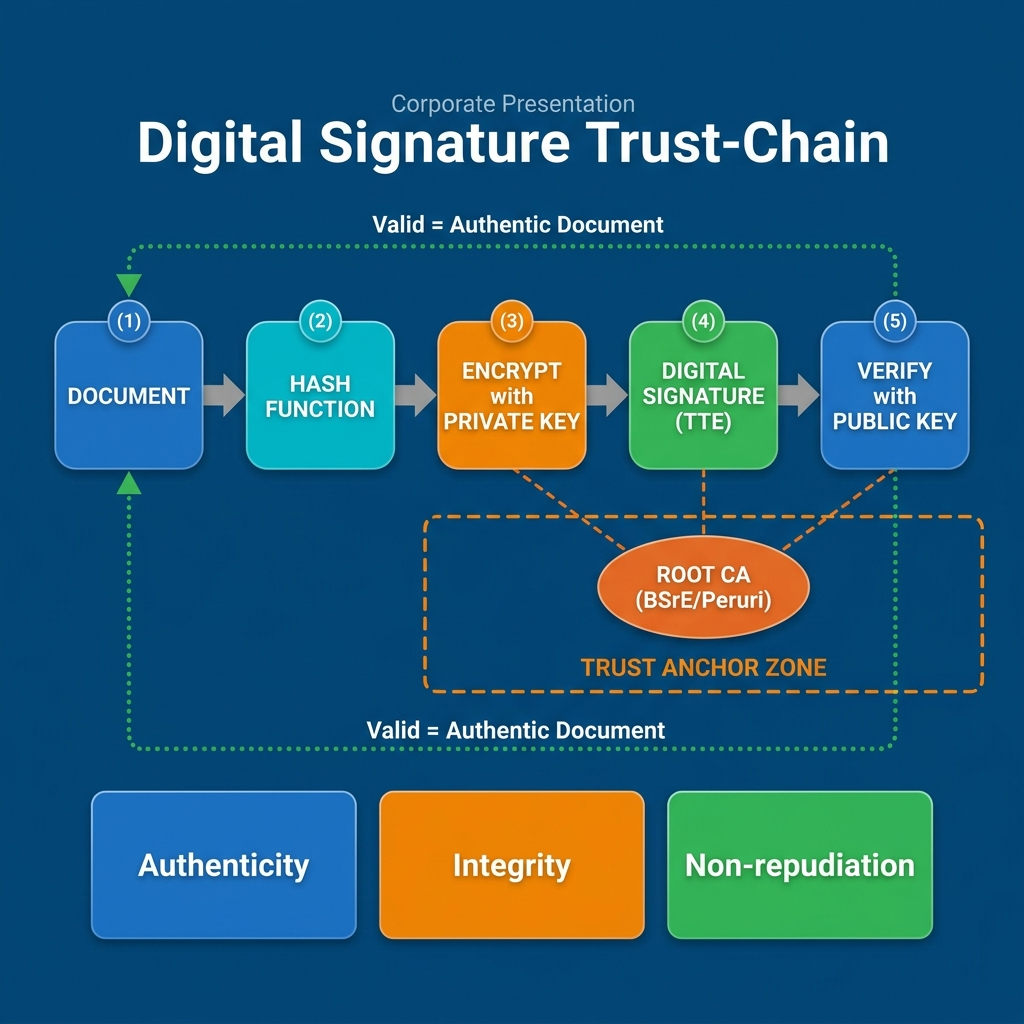
\includegraphics[width=0.7\textwidth]{trust_chain.png}
\caption{Rantai Kepercayaan Tanda Tangan Elektronik: dari Pejabat Penandatangan ke Certificate Authority Terakreditasi}
\end{figure}

\begin{itemize}[leftmargin=*]
    \item Blockchain Hash Chain: Setiap transaksi menghasilkan hash yang menyertakan hash transaksi sebelumnya. Jika satu dokumen diubah, seluruh rangkaian hash menjadi tidak valid dan terdeteksi. Inilah yang disebut \textit{Immutable}.
\end{itemize}

\begin{figure}[H]
\centering
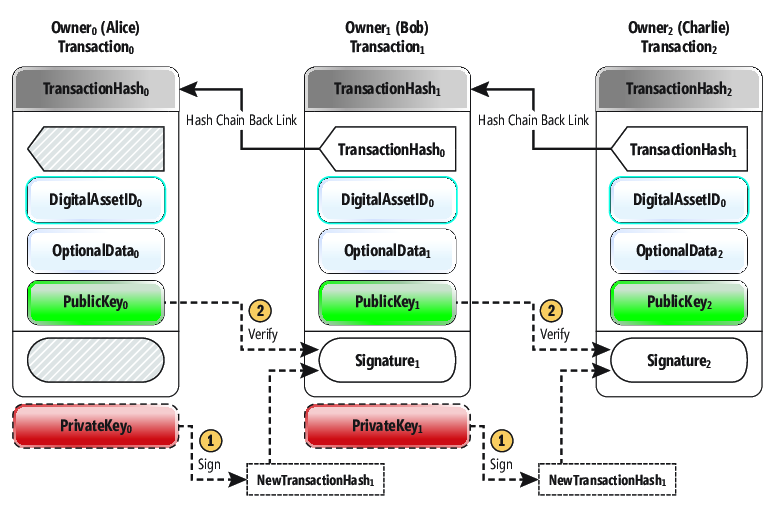
\includegraphics[width=0.65\textwidth]{assets/Blockchain_Hash_Chain.png}
\caption{Rantai Hash untuk Jaminan Immutability: Setiap Transaksi Menyertakan Hash Transaksi Sebelumnya}
\end{figure}

\begin{plnbox}[Ringkasan untuk Manajemen Atas -- Bab 3]
SOP Digital adalah kerangka hukum yang memberikan legitimasi dan keberlanjutan bagi seluruh mekanisme optimalisasi. Tiga pesan kunci: (1) SOP Digital bukan SOP konvensional yang di-scan, melainkan protokol korporat yang mengikat SLA, arsitektur alur kerja, dan kepatuhan regulasi; (2) delapan komponen wajib harus lengkap, khususnya pengakuan \textit{System Custodian} dan dasar hukum digital; dan (3) 14 field metadata adalah \textit{minimum viable} agar arsip memiliki kekuatan hukum menurut regulator.
\end{plnbox}

\needspace{4\baselineskip}

\section{Aktivitas Workshop (30 Menit)}
\textit{(Catatan: Gunakan Lembar Kerja / Form Lampiran yang telah disediakan oleh Instruktur untuk seluruh aktivitas di bawah ini.)}
\begin{enumerate}[leftmargin=*]
    \item Susun draf SOP Digital 8 Komponen untuk 1 proses prioritas (maks. 2 halaman) pada \textbf{Lembar Kerja 1}.
    \item Lengkapi Matriks Metadata 14 Field untuk 1 jenis arsip kritis unit Anda pada \textbf{Lembar Kerja 2}.
    \item Lakukan \textit{peer-review} (validasi silang) atas kelengkapan dasar hukum pada draf rekan Anda.
\end{enumerate}

\begin{outputbox}
Portofolio 3 (Fase 3: SOP Digital): Draft SOP Digital Terintegrasi 8 Komponen + Matriks Metadata 14 Field. Dinilai berdasarkan kelengkapan 8 komponen, kejelasan trigger/SLA, kesesuaian dengan regulasi, dan keberadaan mekanisme fallback.
\end{outputbox}


% ============================================================
\chapter{Justifikasi Bisnis: Efisiensi, ROI \& KPI}
(Kriteria Penilaian 4.3.4 -- Target Kompetensi 4)
% ============================================================

Bab ini mendukung pencapaian Fase 4: Justifikasi Bisnis -- peserta mampu menghitung efisiensi, ROI, dan menyusun justifikasi bisnis berbasis KPI Time-Cost-Risk serta Balanced \textit{scorecard}. 

Setelah SOP Digital (Fase 3) menetapkan dasar operasional dan legal, Manajemen Atas akan dihadapkan pada satu pertanyaan krusial di hadapan dewan direksi atau komite investasi: \textit{``Berapa besar nilai tambah finansial dari transformasi ini?''} Kebijakan dan sistem, walaupun telah lengkap, mustahil disetujui jika tidak didukung oleh pembuktian kelayakan anggaran. Oleh karena itu, justifikasi bisnis (Fase 4) berfungsi sebagai tahap penentu yang mengonversi seluruh perbaikan proses teknis sebelumnya menjadi ukuran pengembalian investasi (ROI) yang kuantitatif.

\needspace{4\baselineskip}

\section{Trifecta Manfaat: Time--Cost--Risk}
Kerangka kerja \textit{Time-Cost-Risk Saving} membagi manfaat transformasi menjadi tiga dimensi:
\begin{itemize}[leftmargin=*]
    \item Time Saving: Pemangkasan waktu tunggu dan durasi proses. Mengukur efisiensi hari ini.
    \item Cost Saving: Reduksi pengeluaran riil (kertas, cetak, ruang, \textit{rework}). Mengukur optimasi anggaran.
    \item Risk Saving: Perlindungan terhadap kerugian finansial masif akibat kehilangan arsip vital atau sanksi hukum. Menjamin keamanan kepatuhan di masa depan.
\end{itemize}

\needspace{4\baselineskip}

\section{Indikator Kinerja Utama (KPI) Target}
\begingroup
\small
\begin{xltabular}{\textwidth}{@{} X X X @{}}
\caption{Indikator Kinerja Utama (KPI) Target Optimalisasi}\\
\toprule
\textbf{Indikator} & \textbf{Definisi} & \textbf{Target Optimasi} \\
\midrule
\endfirsthead

\multicolumn{3}{@{}l}{\small\textit{Lanjutan Tabel \thetable}}\\
\toprule
\textbf{Indikator} & \textbf{Definisi} & \textbf{Target Optimasi} \\
\midrule
\endhead

\bottomrule
\endfoot

\rowcolor{rowalt}
Waktu Siklus (\textit{Cycle Time}) & Waktu total dari draf s.d. tersimpan & Turun 40--60\% \\
Ketepatan Awal (FTA) & \% lolos validasi tanpa revisi & Minimal 90\% \\
\rowcolor{rowalt}
Waktu Temu Kembali & Kecepatan pencarian arsip & $<$ 30 detik (digital) \\
Tingkat Kepatuhan & \% pemenuhan SLA \& regulasi & Minimal 95\% \\
\bottomrule
\end{xltabular}
\endgroup

Penting: Kepatuhan bukan sekadar ``dokumennya ada''. Kepatuhan berarti ada TTE-nya, ada Hash-nya, ada metadata otomatisnya, dan ada audit trail-nya. Itu baru patuh.

\needspace{4\baselineskip}

\section{Balanced \textit{scorecard} (BSC) Perspective}
Keempat KPI di atas masing-masing mewakili satu perspektif Kaplan \& Norton, sehingga laporan kearsipan bisa disajikan sebagai pencapaian korporat:
\begin{itemize}[leftmargin=*]
    \item Financial: \textit{Cost Saved} (dari eliminasi manual \& rework).
    \item Customer: \textit{First-Time Accuracy} (unit kerja lain adalah ``pelanggan'' data kita).
    \item Internal Process: \textit{Cycle Time} (kecepatan alur kerja).
    \item Learning \& Growth: \textit{Compliance Status} (kematangan tata kelola).
\end{itemize}

\begin{figure}[H]
\centering
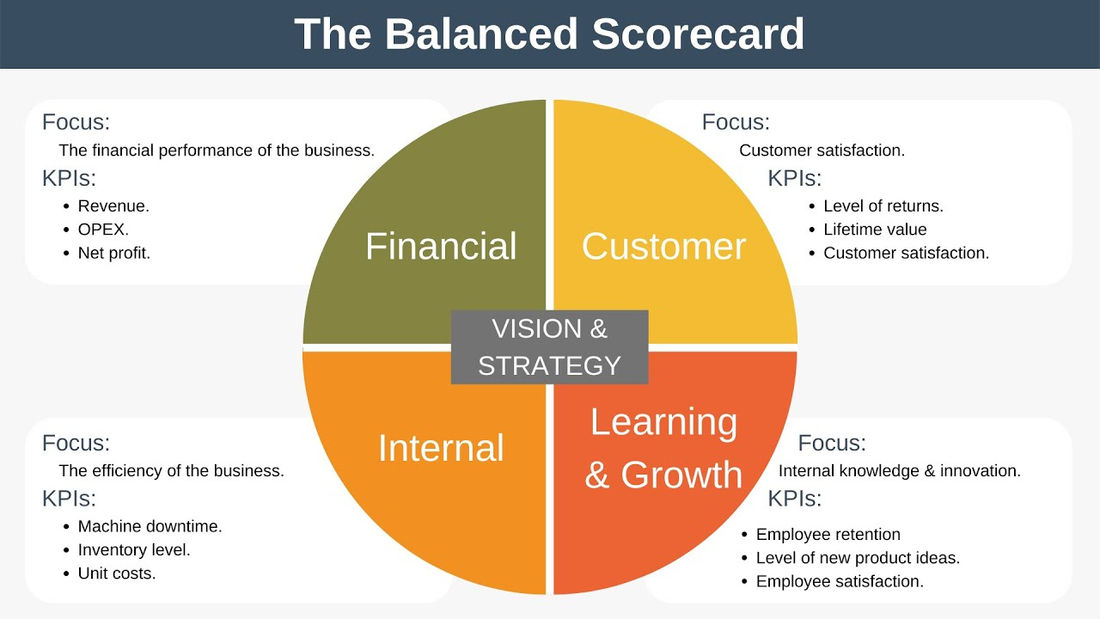
\includegraphics[width=0.75\textwidth]{assets/Balanced_Scorecard.png}
\caption{Balanced \textit{scorecard} Perspective: Memetakan KPI Kearsipan ke Visi Korporat (Sumber: Kaplan \& Norton, 1992)}
\end{figure}

\needspace{4\baselineskip}

\section{Rumus ROI \& Basis Kalkulasi}

Transformasi digital kearsipan memerlukan investasi---baik berupa pengadaan sistem, pelatihan personel, maupun perubahan infrastruktur. Manajemen Atas harus mampu membuktikan bahwa investasi tersebut menghasilkan penghematan atau peningkatan \textit{value} yang terukur. Bagian ini menyajikan rumus ROI yang disederhanakan khusus untuk proyek kearsipan digital, dengan contoh kalkulasi konkret berbasis data operasional PLN yang dapat langsung disesuaikan dengan kondisi unit Anda.
\[
\text{ROI} = \frac{(\Delta \text{Waktu} \times \text{Volume Tahunan} \times \text{Biaya SDM/Jam}) - \text{Biaya Implementasi}}{\text{Biaya Implementasi}} \times 100\%
\]

\noindent Transparansi asumsi diperlukan agar business case dapat dipertanggungjawabkan di depan komite investasi.

\begingroup
\small
\begin{xltabular}{\textwidth}{@{} X X r @{}}
\caption{Asumsi \& Basis Kalkulasi Studi Kasus (Ilustrasi)}\\
\toprule
\textbf{Komponen Kerugian} & \textbf{Basis Perhitungan} & \textbf{Nilai} \\
\midrule
\endfirsthead

\multicolumn{3}{@{}l}{\small\textit{Lanjutan Tabel \thetable}}\\
\toprule
\textbf{Komponen Kerugian} & \textbf{Basis Perhitungan} & \textbf{Nilai} \\
\midrule
\endhead

\bottomrule
\endfoot

\rowcolor{rowalt}
Waktu siklus terbuang & 1.200 arsip $\times$ 4,2 hari $\times$ Rp 150.000/hari & Rp 756 jt \\
Biaya revisi metadata & 420 arsip gagal $\times$ 2 jam $\times$ Rp 62.500/jam & Rp 52,5 jt \\
\rowcolor{rowalt}
Kehilangan arsip vital & 8 kasus $\times$ Rp 25 jt (rekonstruksi + sanksi) & Rp 200 jt \\
Temu kembali lambat & 1.200 arsip $\times$ 0,25 jam $\times$ Rp 125.000/jam & Rp 37,5 jt \\
\midrule
\multicolumn{2}{@{}l}{\textbf{Total Estimasi Kerugian}} & \textbf{Rp 1.046.000.000} \\
\bottomrule
\end{xltabular}
\endgroup

\begin{plnbox}[Parameter yang Harus Disesuaikan per Unit]
Ganti angka-asumsi di atas dengan data faktual unit Anda: (1) Volume arsip/tahun, (2) Rata-rata frekuensi kehilangan, (3) Biaya tenaga kerja lokal, dan (4) Waktu siklus aktual. Logika kalkulasi tetap sama.
\end{plnbox}

\begin{figure}[H]
\centering
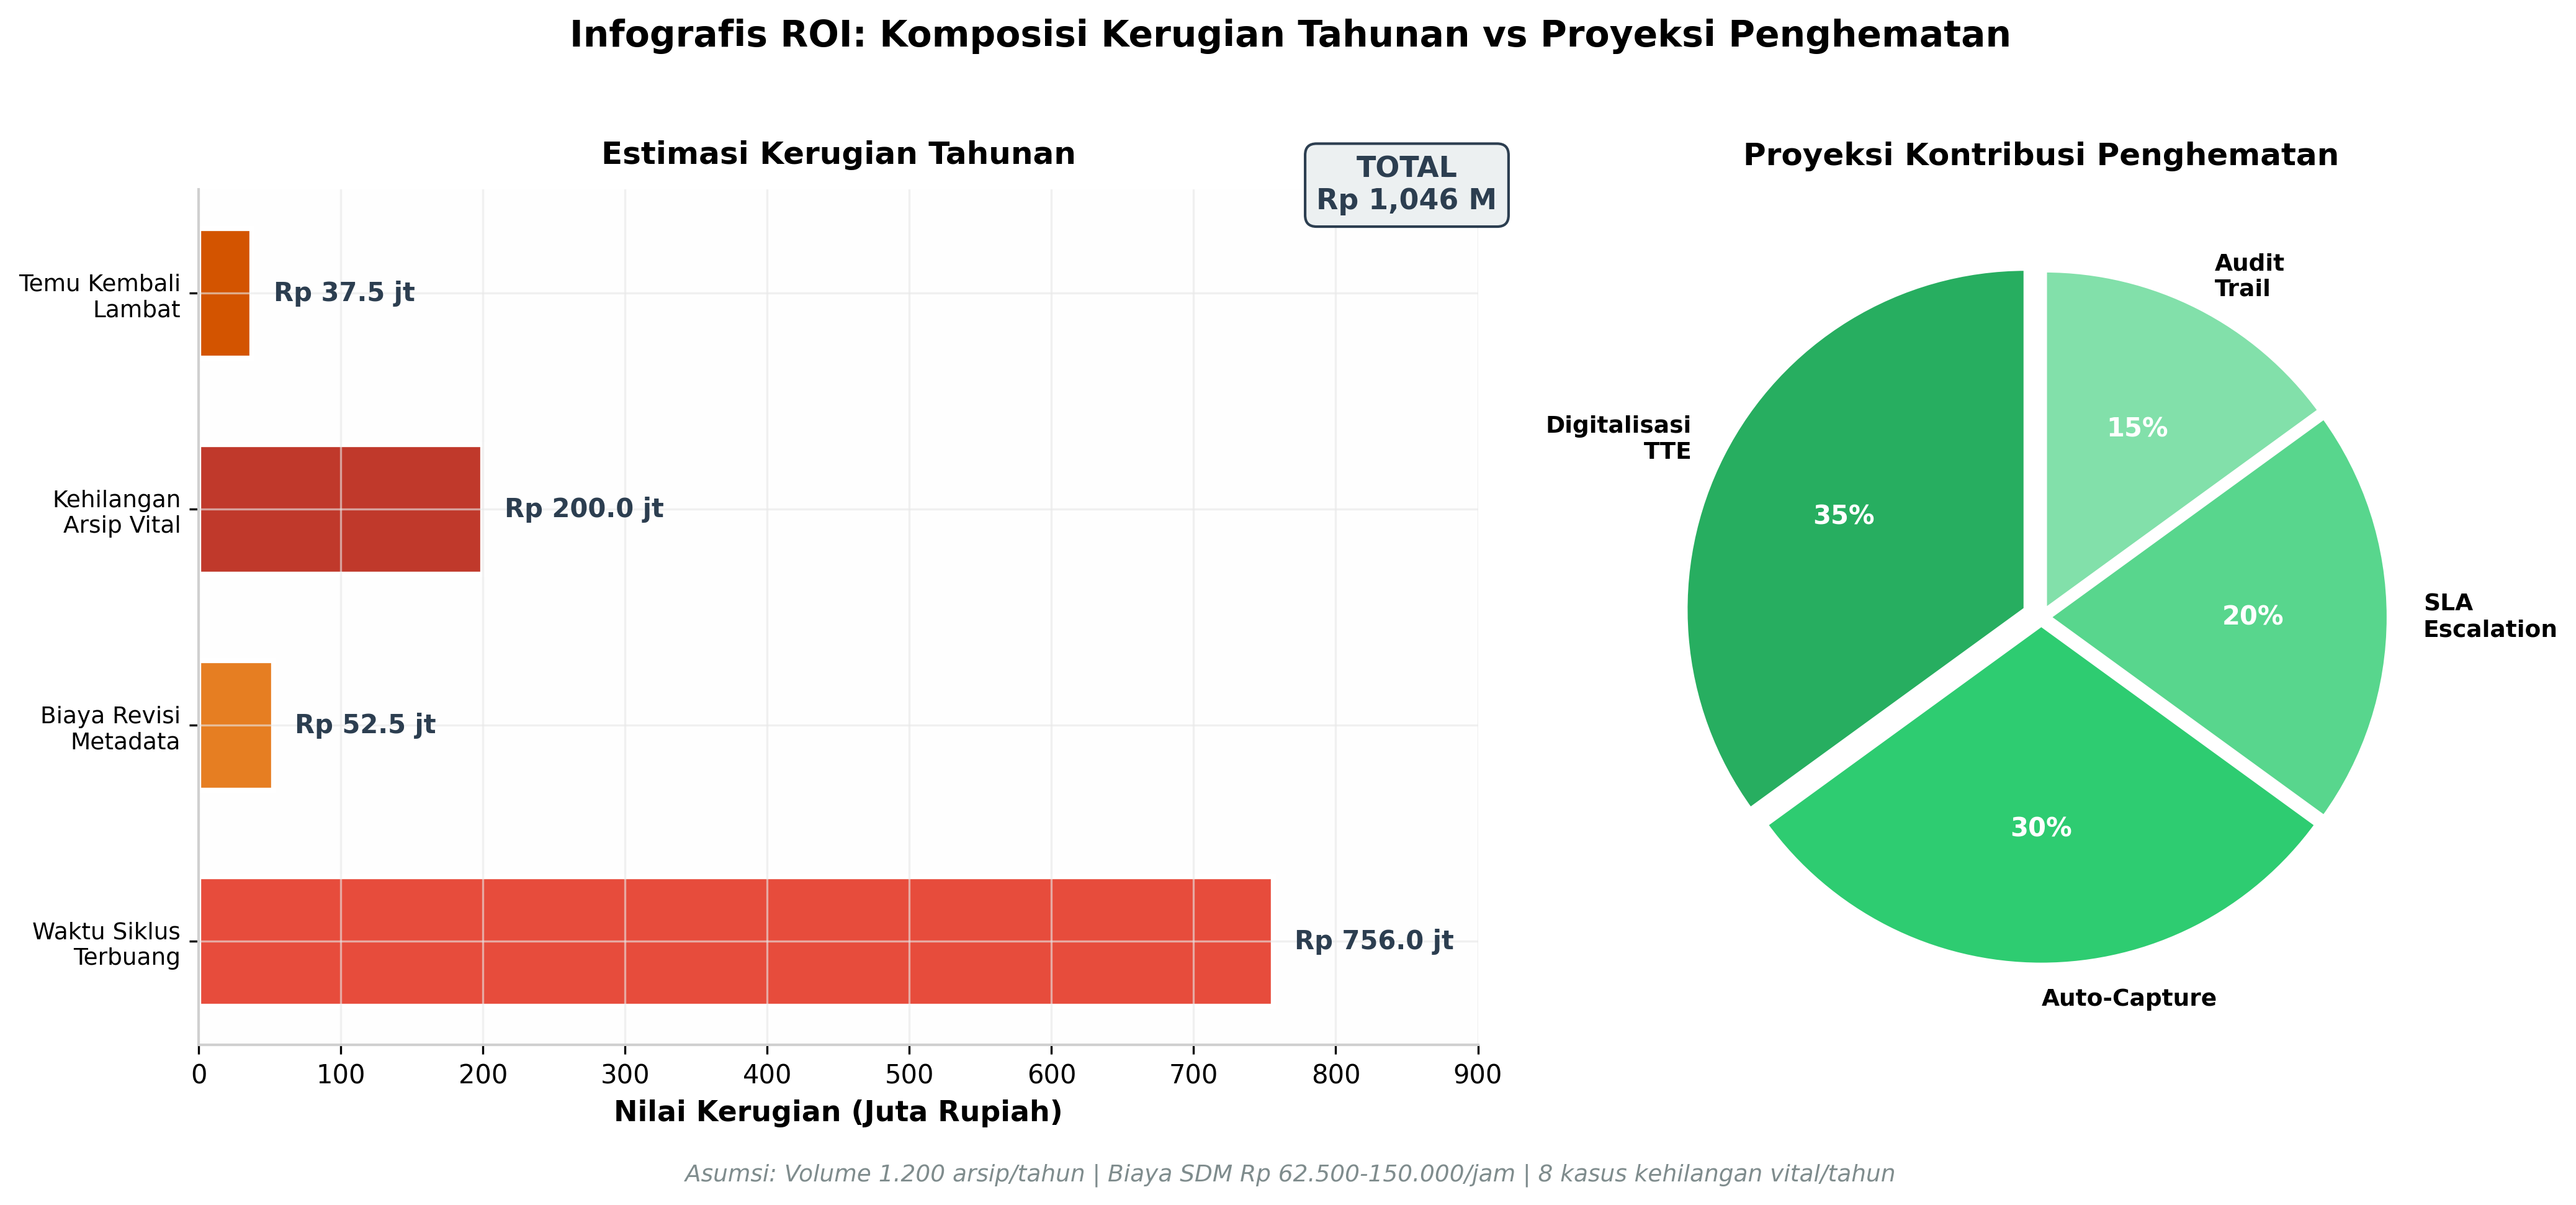
\includegraphics[width=0.95\textwidth]{assets/infografis_roi.png}
\caption{Infografis ROI: Komposisi Kerugian Tahunan (Rp 1,046 Miliar) dan Proyeksi Kontribusi Penghematan}
\end{figure}

\needspace{4\baselineskip}

\section{Studi Kasus: Transformasi SPK Pemeliharaan GI 150 kV}
Profil Unit: UIT Jawa Bagian Tengah -- 48 Gardu Induk 150 kV -- Volume 1.200 SPK/tahun.

Kondisi \textit{as-is} (Hasil Pemodelan):
\begin{itemize}[leftmargin=*]
    \item Waktu siklus rata-rata: 5 hari
    \item Kesalahan metadata: 35\% (420 dokumen/tahun perlu revisi, 2 jam/revisi)
    \item Kehilangan arsip: 8 kasus/tahun
    \item Waktu temu kembali: 15--30 menit (fisik)
    \item Total estimasi kerugian: Rp 1.046.000.000/tahun
\end{itemize}

Intervensi: Trigger-Based Auto-Capture, Parallel Digital Routing, SLA-Driven Escalation, Hash-Lock Immutable, pembaruan SOP.

Kondisi \textit{to-be} (Setelah 90 Hari Pilot):
\begin{itemize}[leftmargin=*]
    \item Waktu siklus: 0,8 hari (turun 84\%)
    \item Ketepatan Awal: 100\% (dari 65\%)
    \item Waktu temu kembali: $<$20 detik (turun 99\%)
    \item Tingkat Kepatuhan: 98\% (dari 72\%)
    \item Kehilangan arsip / Temuan audit BPK: 0
\end{itemize}

\begin{figure}[H]
\centering
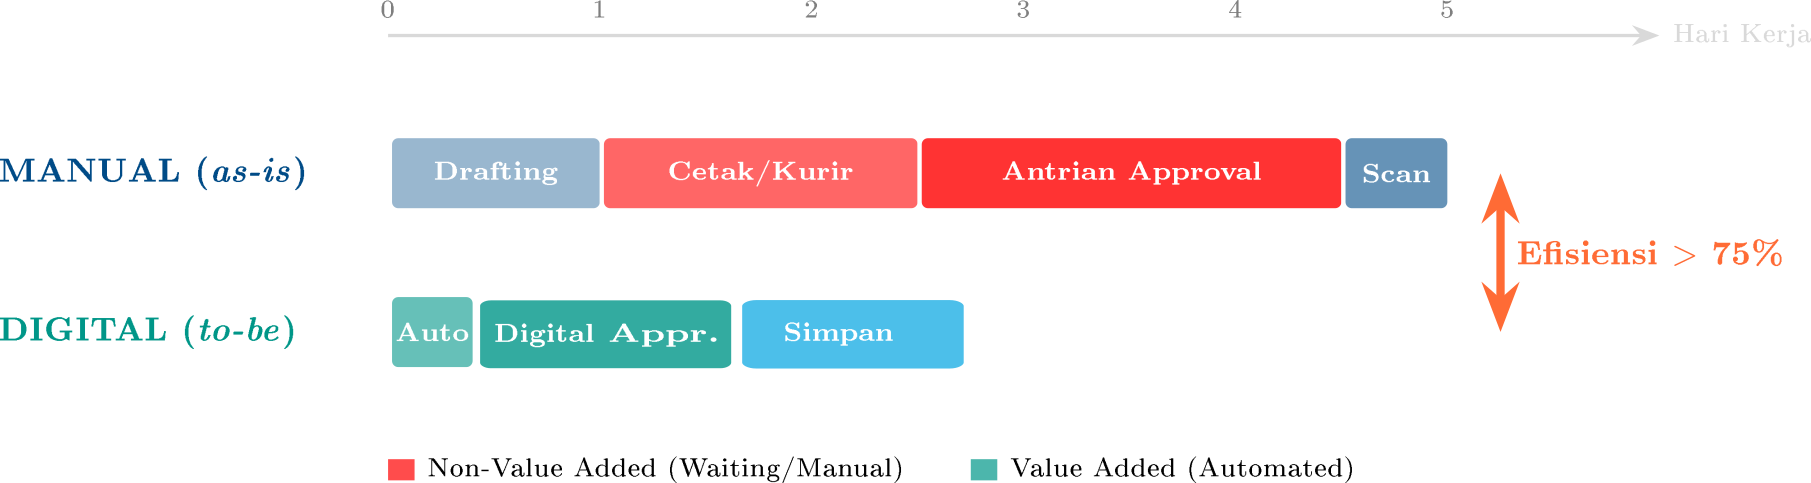
\includegraphics[width=0.9\textwidth]{assets/efficiency_heatmap.png}
\caption{Efficiency Heatmap: Perbandingan Durasi Siklus Manual vs Digital}
\end{figure}

\textit{Analisis:} Proses manual diwakili oleh linimasa panjang dengan hambatan operasional. Proses digital diwakili oleh linimasa efisien yang difokuskan pada aktivitas \textit{Value Added}.

Kalkulasi ROI (Simulasi):
\begin{itemize}[leftmargin=*]
    \item Total Manfaat Tahunan: Rp 1.046.000.000
    \item Total Biaya Tahun Pertama: Rp 161.000.000
    \item Keuntungan Bersih: Rp 885.000.000
    \item ROI: 550\% --- Payback Period: $<$ 2 bulan
\end{itemize}

\begin{plnbox}[Ringkasan untuk Manajemen Atas -- Bab 4]
Justifikasi bisnis adalah dasar legitimasi anggaran: tanpa bukti kuantitatif, transformasi tidak akan mendapatkan persetujuan komite investasi. Tiga pesan kunci: (1) gunakan kerangka Time-Cost-Risk untuk memastikan tidak ada dimensi manfaat yang terlupakan; (2) KPI harus dipetakan ke Balanced \textit{scorecard} agar dapat disajikan sebagai pencapaian korporat; dan (3) transparansi asumsi adalah prasyarat akuntabilitas -- jangan sembunyikan angka-asumsi di balik total akhir.
\end{plnbox}

\needspace{4\baselineskip}

\section{Aktivitas Workshop (30 Menit)}
\textit{(Catatan: Gunakan \textbf{Lampiran D: Business Case \& Action Plan 30 Hari} untuk aktivitas ini.)}
\begin{enumerate}[leftmargin=*]
    \item Pilih 1 proses prioritas dari unit Anda dan kalkulasi estimasi kerugian tahunan (Time-Cost-Risk).
    \item Tetapkan target KPI (Cycle Time, FTA, Compliance) yang realistis.
    \item Susun Business Case 1 halaman dengan estimasi biaya implementasi dan proyeksi ROI.
\end{enumerate}

\begin{outputbox}
Portofolio 4 (Fase 4: Justifikasi Bisnis): Business Case 1 Halaman + Action Plan 30 Hari + KPI Tracker. Dinilai berdasarkan kejelasan kalkulasi ROI, realisme asumsi, kesesuaian KPI dengan Balanced \textit{scorecard}, dan kelengkapan Action Plan.
\end{outputbox}


% ============================================================
\chapter{Manajemen Perubahan: Implementasi \& Mitigasi Resistensi}
% ============================================================

Setelah proposal justifikasi bisnis dan penghitungan ROI (Bab 4) disetujui, unit kerja siap bergerak menuju tahap eksekusi implementasi. Namun, sebaik apa pun rancangan alur kerja dan sistem digital yang telah dibuat, penerapannya di lapangan tidak akan berhasil tanpa dukungan penuh dari sumber daya manusia yang mengoperasikannya. 

Oleh karena itu, investasi teknologi harus diawasi ketat oleh strategi \textit{Change Management}. Bab ini tidak sekadar membahas cara melatih pegawai menggunakan aplikasi baru, melainkan sebuah strategi sistematis untuk mengubah resistensi (penolakan) individu menjadi komitmen kolektif terhadap budaya kerja terintegrasi PLN. Pembahasan akan berfokus pada dua kerangka yang paling relevan: ADKAR (untuk transisi individu) dan Kotter (untuk transformasi organisasi).

\begin{warnbox}[Peringatan untuk Manajemen Atas]
Kesalahan paling fatal dalam transformasi digital kearsipan bukan memilih teknologi yang salah, melainkan mengabaikan dimensi manusia. Sebagian besar pilot project yang gagal di lingkungan BUMN bukan karena sistemnya tidak berfungsi, tetapi karena personel tidak disiapkan secara memadai untuk mengadopsinya. Alokasikan minimal 30\% dari anggaran dan waktu implementasi untuk aktivitas manajemen perubahan.
\end{warnbox}

\needspace{4\baselineskip}

\section{Kerangka ADKAR (Hiatt, 2006)}
Lima tahapan perubahan pada level individu:
\begin{enumerate}[leftmargin=*]
    \item Awareness: Bangun kesadaran bahwa prosedur manual saat ini punya ``biaya tersembunyi'' yang menurunkan efisiensi.
    \item Desire: Tumbuhkan kemauan dengan menunjukkan \textit{\textit{quick win}} dalam 30 hari pertama.
    \item Knowledge: Berikan pelatihan teknis yang fokus pada manfaat, bukan tombol.
    \item Ability: Pastikan mampu mengoperasikan melalui pendampingan personal.
    \item Reinforcement: Jaga agar perubahan bertahan melalui SKI, audit, dan insentif.
\end{enumerate}

\begin{figure}[H]
\centering
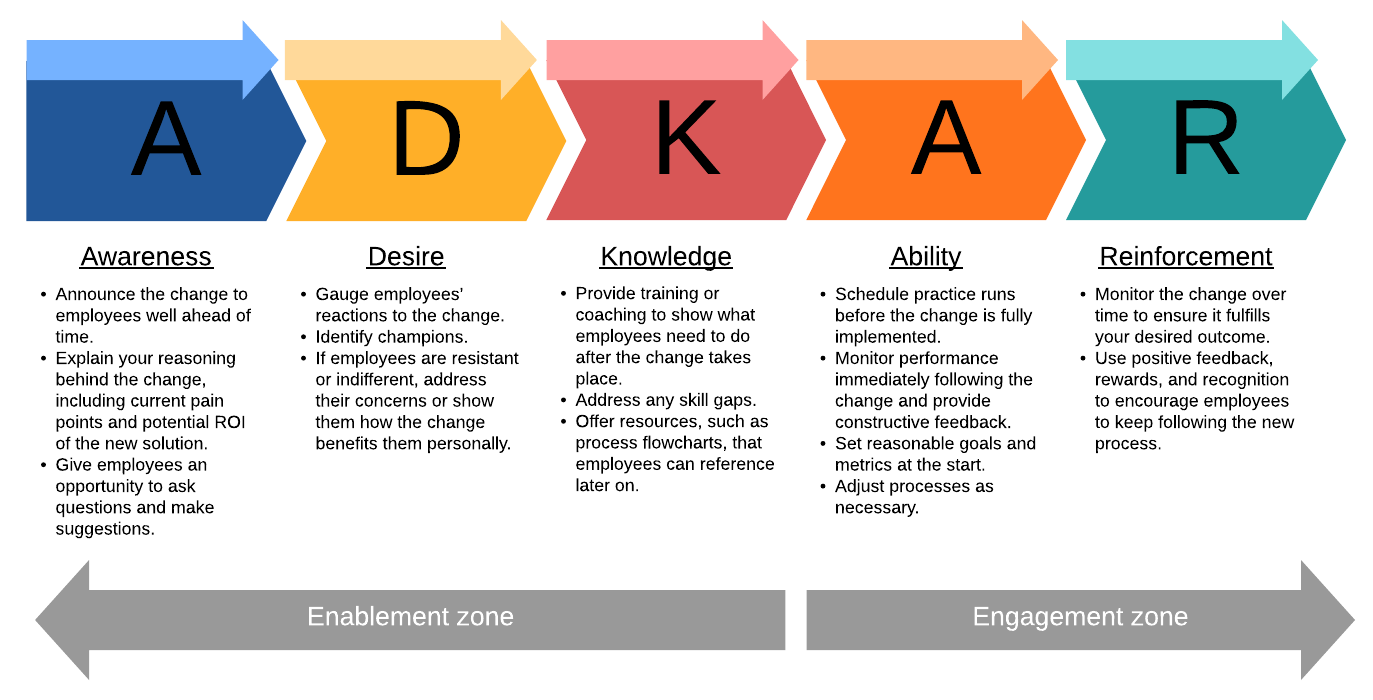
\includegraphics[width=0.7\textwidth]{assets/ADKAR_Model.png}
\caption{Model ADKAR: Lima Tahapan Perubahan pada Level Individu (Sumber: Hiatt, 2006)}
\end{figure}

\needspace{4\baselineskip}

\section{Kotter: 3 Langkah Kepemimpinan yang Paling Relevan}
Dari 8 langkah Kotter (1996), tiga yang paling krusial untuk konteks PLN:
\begin{itemize}[leftmargin=*]
    \item Membentuk Koalisi: Bentuk \textit{Duta Kearsipan} di setiap unit --- supervisor muda yang menjadi pelaksana praktik terbaik.
    \item Capaian Jangka Pendek (\textit{quick win}): Pilot 30 hari pertama harus menunjukkan hasil konkret (misal: ``waktu siklus berkurang 90\% di GI X'').
    \item Penguatan Budaya: Pelembagaan melalui SKI, audit berkala, dan transparansi \textit{dashboard}.
\end{itemize}

\textit{Pesan kunci:} Kalau pimpinan masih minta staf mencetak draf agar bisa dibaca di kertas, maka pimpinan menunjukkan ketidakpercayaan terhadap sistem digital. Pimpinan harus jadi pengguna pertama.

\begin{figure}[H]
\centering
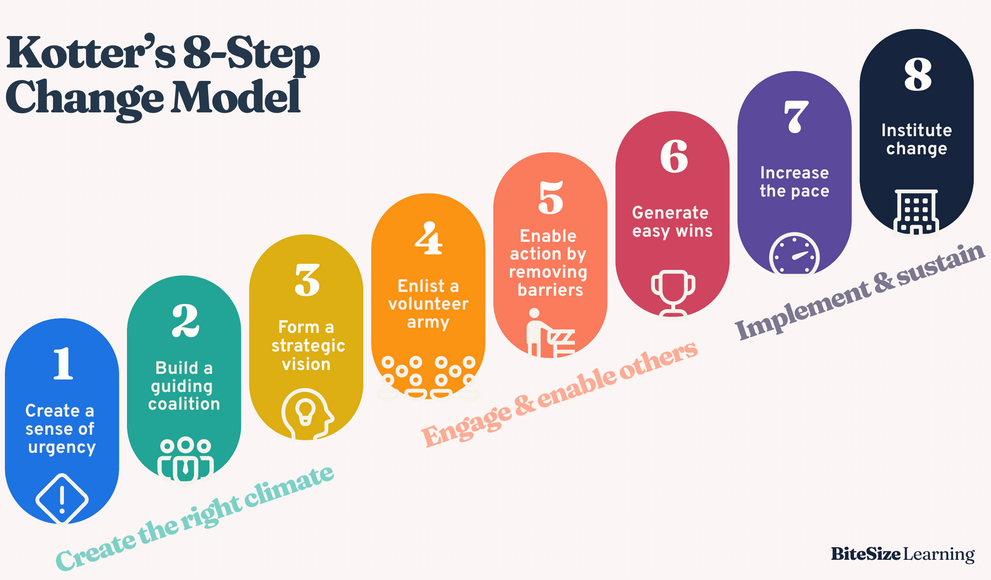
\includegraphics[width=0.75\textwidth]{assets/Kotters_8_Step.png}
\caption{Model Kotter 8 Step: Kerangka Kepemimpinan Transformasi (Sumber: Kotter, 1996)}
\end{figure}

\needspace{4\baselineskip}

\section{Matriks Strategi Mitigasi Resistensi}
\begingroup
\small
\begin{xltabular}{\textwidth}{@{} l X X @{}}
\caption{Matriks Mitigasi Resistensi: Pola Perilaku \& Taktik Manajerial}\\
\toprule
\textbf{Jenis Resistensi} & \textbf{Pola Perilaku} & \textbf{Taktik Manajerial} \\
\midrule
\endfirsthead

\multicolumn{3}{@{}l}{\small\textit{Lanjutan Tabel \thetable}}\\
\toprule
\textbf{Jenis Resistensi} & \textbf{Pola Perilaku} & \textbf{Taktik Manajerial} \\
\midrule
\endhead

\bottomrule
\endfoot

\rowcolor{rowalt}
Kebiasaan & ``Cara lama sudah berjalan baik, kenapa harus berubah?'' & Tunjukkan \textit{\textit{quick win}} hasil pilot $<$30 hari. \\
Kompetensi & ``Saya tidak mengerti teknologi ini.'' & Pendampingan personal dan \textit{peer-learning}. \\
\rowcolor{rowalt}
Kewenangan & ``Ini mengubah siapa yang memutuskan apa.'' & Berikan peran sebagai \textit{Duta Kearsipan} --- akui pengalaman mereka. \\
Kepercayaan & ``Tanda tangan basah lebih sah secara hukum.'' & Sosialisasi PP 71/2019 \& demonstrasi audit trail digital yang justru lebih melindungi. \\
\rowcolor{rowalt}
Data Efisiensi & ``Angka-angka itu hanya teori.'' & Tampilkan data efisiensi hasil pilot di rapat manajemen rutin secara transparan. \\
\bottomrule
\end{xltabular}
\endgroup

\needspace{4\baselineskip}

\section{Matriks Mendelow: Power vs Interest}
Gunakan matriks ini untuk memprioritaskan strategi komunikasi:
\begin{itemize}[leftmargin=*]
    \item Kuadran Kanan Atas (Power Tinggi, Interest Tinggi): GM, VP, Manajer Area. \textit{Kelola secara intensif} --- mereka berpengaruh langsung pada keberhasilan proyek.
    \item Kuadran Kiri Atas (Power Tinggi, Interest Rendah): Penyelia Senior, Auditor. \textit{Jaga kepuasan} --- kalau tidak puas, mereka bisa jadi penghambat.
    \item Kuadran Kanan Bawah (Power Rendah, Interest Tinggi): Tim IT, Unit Kearsipan. \textit{Mitra kerja teknis} --- libatkan dalam desain detail.
    \item Kuadran Kiri Bawah (Power Rendah, Interest Rendah): Staf operasional umum. \textit{Pantau minimal} --- beri informasi rutin.
\end{itemize}

\begin{figure}[H]
\centering
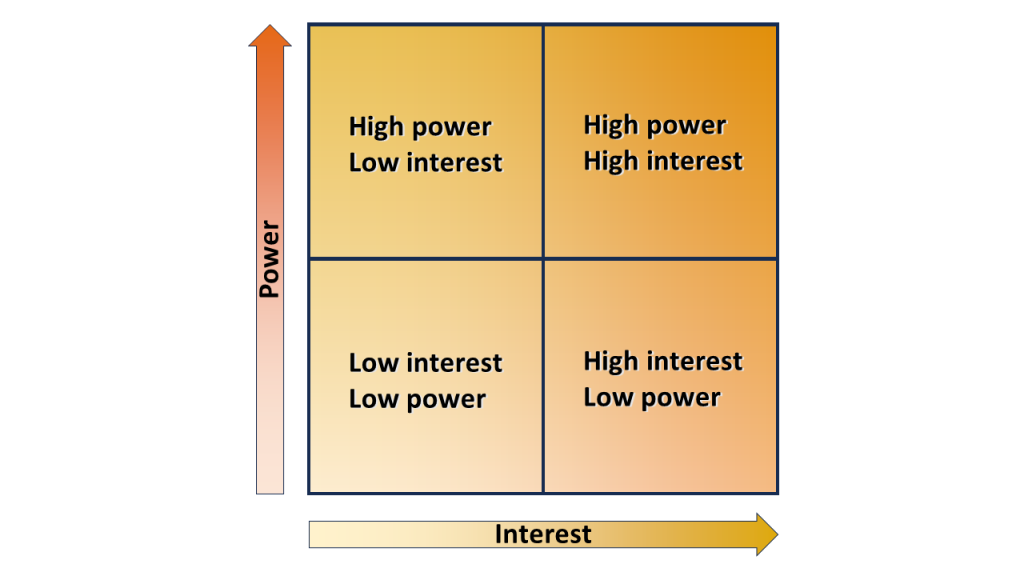
\includegraphics[width=0.65\textwidth]{assets/Power-Interest_Grid.png}
\caption{Matriks Mendelow (Power/Interest Grid): Panduan Prioritisasi Stakeholder}
\end{figure}

\needspace{4\baselineskip}

\section{Taktik 30 Hari Pertama yang Terbukti Efektif}
\begin{enumerate}[leftmargin=*]
    \item Minggu 1--2: Parallel Run. Jalankan proses lama dan baru secara bersamaan. Jangan langsung matikan cara lama. Biarkan staf melihat sendiri bahwa cara digital lebih cepat.
    \item Minggu 3: Cut-Off. Hentikan proses lama secara resmi setelah staf merasa percaya diri. Sediakan \textit{helpdesk} internal untuk pertanyaan cepat.
    \item Minggu 4: Rayakan \textit{quick win}. Publikasikan data ``arsip diproses dalam 4 jam vs sebelumnya 5 hari'' di forum internal/grup koordinasi unit.
\end{enumerate}
Kunci sukses: Jangan pernah mempermalukan personel yang lambat beradaptasi. Gunakan pendekatan \textit{``kita belajar bersama''}.

\needspace{4\baselineskip}

\section{7 Kesalahan Umum yang Harus Dihindari}

Bagian ini dirancang khusus untuk membantu Manajemen Atas mengenali \textit{red flags} --- tanda-tanda kegagalan yang sering terjadi pada proyek transformasi digital kearsipan. Ketujuh kesalahan berikut bukanlah daftar teknis semata, melainkan refleksi dari kegagalan nyata di berbagai organisasi BUMN dan instansi pemerintah. Memahami dan mengantisipasinya akan menghemat anggaran, mengurangi risiko audit, serta mempercepat pencapaian \textit{value} dari investasi teknologi yang telah disetujui.
\begin{enumerate}[leftmargin=*]
    \item ``Cepat = Berkualitas'' --- Tanpa metadata otomatis, hash integrity, dan audit trail, dokumen cepat hanyalah ``file tanpa konteks'' yang tidak memenuhi syarat hukum.
    \item ``SOP Digital = User Guide Aplikasi'' --- SOP Digital adalah protokol korporat, bukan buku panduan klik tombol.
    \item Parallel Routing tanpa Immutability Lock --- Tanpa penguncian \textit{read-only}, revisi berbarengan akan memicu \textit{version conflict}.
    \item ``Integrasi = Koneksi API Antar-Server'' --- Integrasi sistem kearsipan bukan sekadar menyambungkan koneksi API antar-server milik IT, melainkan penciptaan ekosistem tata kelola di mana data, struktur, dan konteks dokumen berpindah secara utuh tanpa intervensi tangan manusia.
    \item ``100\% Paperless atau Tidak Sama Sekali'' --- Transformasi digital kearsipan bukan sekadar tekanan agar organisasi menjadi 100\% \textit{paperless} dalam semalam, melainkan membangun sinkronisasi presisi antara repositori fisik dan \textit{Finding Aid} digital demi kepastian hukum.
    \item Mendelegasikan Validasi BPMN Mutlak ke IT/Vendor --- BPMN adalah rancangan arsitektur hukum. Tanpa validasi bisnis, sistem bisa berujung pada pelanggaran wewenang persetujuan.
    \item ``Metadata Hanya Nomor Dokumen dan Tanggal'' --- Metadata bukan sekadar daftar nomor dokumen dan tanggal pembuatan, melainkan matriks keamanan yang secara absolut menentukan keabsahan hukum, mengeksekusi retensi otomatis, dan mengunci hak akses (RBAC) arsip Anda.
\end{enumerate}

\begin{plnbox}[Ringkasan untuk Manajemen Atas -- Bab 5]
Manajemen perubahan adalah prasyarat keberhasilan implementasi: tanpa dukungan personel, teknologi terbaik pun akan gagal. Tiga pesan kunci: (1) alokasikan minimal 30\% anggaran untuk manajemen perubahan; (2) pimpinan harus menjadi pengguna pertama sistem digital; dan (3) jangan pernah mempermalukan staf yang lambat beradaptasi -- gunakan pendekatan ``kita belajar bersama''.
\end{plnbox}


% ============================================================
\chapter{Validasi, Rubrik Penilaian \& Komitmen Tindak Lanjut}
% ============================================================

Seluruh tahapan dari Fase Diagnosa di awal hingga mitigasi SDM di Bab 5 pada akhirnya akan berujung pada satu momen esensial: \textit{Persetujuan Eksekutif}. Bab penutup ini menyajikan kerangka validasi akhir guna memastikan bahwa setiap dokumen portofolio yang diajukan sudah benar-benar memenuhi kelayakan operasional PLN.

\needspace{4\baselineskip}

\section{Executive Tollgate Final (4 Gerbang Keputusan)}

Sebelum membubuhkan tanda tangan persetujuan \textit{go-live} yang akan mengkomitkan pengeluaran anggaran, Manajemen Atas memerlukan kerangka verifikasi yang tidak dapat ditawar. \textit{Executive Tollgate} hadir bukan sebagai formalitas administratif belaka, melainkan sebagai instrumen perlindungan berlapis untuk meniadakan risiko kegagalan proyek. Pastikan keempat gerbang keputusan berikut seluruhnya berstatus hijau sebelum investasi kearsipan digital tersebut resmi dieksekusi:

\begingroup
\small
\begin{xltabular}{\textwidth}{@{} l X @{}}
\caption{Executive Tollgate Final: Empat Gerbang Keputusan Implementasi}\\
\toprule
\textbf{Gerbang} & \textbf{Pertanyaan Kunci} \\
\midrule
\endfirsthead

\multicolumn{2}{@{}l}{\small\textit{Lanjutan Tabel \thetable}}\\
\toprule
\textbf{Gerbang} & \textbf{Pertanyaan Kunci} \\
\midrule
\endhead

\bottomrule
\endfoot

\rowcolor{rowalt}
1. Legal Compliance & Apakah alur baru selaras dengan pedoman tata naskah dan regulasi nasional? \\
2. Data Integrity & Apakah audit trail, TTE, \& Hash SHA-256 sudah menjamin keaslian? \\
\rowcolor{rowalt}
3. Operational Value & Apakah efisiensi waktu \& biaya sudah tervalidasi melalui kalkulasi ROI? \\
4. Scalability & Apakah infrastruktur IT siap untuk volume data jangka panjang? \\
\bottomrule
\end{xltabular}
\endgroup

\textit{Kalau ada gerbang yang masih merah, mundur satu langkah --- evaluasi ulang di bagian diagnosa atau desain SOP. Jangan pernah memaksakan implementasi yang belum siap.}

\needspace{4\baselineskip}

\section{Rubrik Penilaian \& \textit{checklist} Portofolio}
Peserta dinyatakan lulus Modul 4.3 jika memenuhi kriteria berikut:

\begingroup
\small
\begin{xltabular}{\textwidth}{@{} l X c @{}}
\caption{Rubrik Penilaian \& \textit{checklist} Kelulusan Modul 4.3}\\
\toprule
\textbf{No} & \textbf{Komponen Penilaian} & \textbf{Status} \\
\midrule
\endfirsthead

\multicolumn{3}{@{}l}{\small\textit{Lanjutan Tabel \thetable}}\\
\toprule
\textbf{No} & \textbf{Komponen Penilaian} & \textbf{Status} \\
\midrule
\endhead

\bottomrule
\endfoot

\rowcolor{rowalt}
1 & Matriks Identifikasi Area Optimasi (minimal 4 area, lengkap dengan hambatan \& prioritas) & $\square$ \\
2 & Diagram BPMN 2.0 \textit{to-be} + Peta Pemicu Integrasi & $\square$ \\
\rowcolor{rowalt}
3 & Draft SOP Digital Terintegrasi (8 komponen lengkap) & $\square$ \\
4 & Business Case 1 Halaman + Action Plan 30 Hari + KPI Tracker & $\square$ \\
\midrule
\rowcolor{plnblue!15}
5 & Skor Rubrik Penilaian Terintegrasi $\geq$ 70/100 & $\square$ \\
6 & Post-Test Konseptual LMS PLN $\geq$ 65/100 & $\square$ \\
\rowcolor{plnblue!15}
7 & Komitmen Tindak Lanjut Implementasi (tertulis \& ditandatangani) & $\square$ \\
\bottomrule
\end{xltabular}
\endgroup

\textit{Target Akhir: Empat dokumen portofolio menjadi blueprint transformasi yang dapat langsung diusulkan sebagai pilot project di unit kerja masing-masing.}

\needspace{4\baselineskip}

\section{\textit{checklist} Implementasi 30 Hari}
\begingroup
\small
\begin{xltabular}{\textwidth}{@{} l X X l @{}}
\caption{Rencana Aksi Implementasi 30 Hari}\\
\toprule
\textbf{Minggu} & \textbf{Aktivitas Utama} & \textbf{Sasaran} & \textbf{PIC} \\
\midrule
\endfirsthead

\multicolumn{4}{@{}l}{\small\textit{Lanjutan Tabel \thetable}}\\
\toprule
\textbf{Minggu} & \textbf{Aktivitas Utama} & \textbf{Sasaran} & \textbf{PIC} \\
\midrule
\endhead

\bottomrule
\endfoot

\rowcolor{rowalt}
Minggu 1 & Pilot Launch & Integrasi API, pelatihan tim percontohan & $\ldots$ \\
Minggu 2 & Parallel Run & Jalankan proses lama dan baru bersamaan; biarkan staf melihat sendiri & $\ldots$ \\
\rowcolor{rowalt}
Minggu 3 & Cut-Off Resmi & Hentikan proses lama; sediakan helpdesk untuk pertanyaan & $\ldots$ \\
Minggu 4 & Standardisasi & Evaluasi KPI, publikasikan data efisiensi, persiapkan replikasi ke unit lain & $\ldots$ \\
\bottomrule
\end{xltabular}
\endgroup

\needspace{4\baselineskip}

\section{FAQ Singkat untuk Manajemen Atas}

\begin{plnbox}[Q: Apakah TTE Tersertifikasi setara dengan tanda tangan basah?]
A: Ya. Sesuai Pasal 14--16 PP 71/2019, TTE Tersertifikasi memiliki kekuatan hukum dan akibat hukum yang sama persis dengan tanda tangan basah. SOP yang mengimplementasikannya memiliki \textit{legal standing} tak terbantahkan.
\end{plnbox}

\begin{plnbox}[Q: Bagaimana jika sistem down saat proses berlangsung?]
A: Komponen ke-7 SOP Digital (Exception \& Fallback) mewajibkan adanya prosedur \textit{fallback}. Dokumen ditahan di \textit{Waiting Terminal} dengan \textit{alert} ke IT. Tidak ada dokumen disahkan melalui ``proses luring tanpa pencatatan.''
\end{plnbox}

\begin{plnbox}[Q: Apakah ini berarti 100\% paperless?]
A: Tidak selalu. Organisasi infrastruktur besar masih dalam masa transisi Arsip Hibrida. Jika regulasi mensyaratkan fisik, yang diotomasi adalah \textit{metadata tracking} dan sinkronisasi depo arsip fisik dengan \textit{Finding Aid} digital.
\end{plnbox}

\begin{plnbox}[Q: Mengapa Manajemen Atas harus ikut mempelajari BPMN?]
A: MA tidak perlu menggambar dari nol, tetapi wajib bisa membaca, memvalidasi, dan mengesahkan diagram. BPMN adalah rancangan arsitektur hukum proses. Tanpa validasi MA, sistem buatan IT bisa berujung pada pelanggaran wewenang persetujuan atau kebocoran akses.
\end{plnbox}

\needspace{4\baselineskip}

\section{Empat Langkah Setelah Hari Ini}
\begin{enumerate}[leftmargin=*]
    \item Identifikasi 1 proses prioritas di unit Anda dalam 7 hari.
    \item Bentuk koalisi mini (IT + Unit Kearsipan + Manajer Area).
    \item Jalankan Parallel Run selama 2 minggu pada proses terpilih.
    \item Laporkan \textit{quick win} pertama ke atasan dengan data ROI awal.
\end{enumerate}

\begin{plnbox}[Komitmen Saya]
\vspace{0.3cm}
Saya berjanji akan menginisiasi optimalisasi pada proses \dotfill dengan target penurunan waktu siklus sebesar \dotfill \% pada tanggal \dotfill.

\vspace{1.2cm}
\begin{flushright}
\begin{minipage}{0.5\textwidth}
\centering
\dotfill\\
Nama \& Jabatan
\end{minipage}
\end{flushright}
\end{plnbox}


% ============================================================
\chapter*{Glosarium}
\addcontentsline{toc}{chapter}{Glosarium}
% ============================================================

\begingroup
\small
\begin{xltabular}{\textwidth}{@{} >{\bfseries}l X @{}}
\caption{Glosarium: Istilah Teknis dalam Manajemen Arsip Digital}\\
\toprule
\textbf{Istilah} & \textbf{Definisi} \\
\midrule
\endfirsthead

\multicolumn{2}{@{}l}{\small\textit{Lanjutan Tabel}}\\
\toprule
\textbf{Istilah} & \textbf{Definisi} \\
\midrule
\endhead

\bottomrule
\endfoot

ADKAR & Model perubahan individu (Awareness, Desire, Knowledge, Ability, Reinforcement). \\
ANRI & Arsip Nasional Republik Indonesia. \\
BAST & Berita Acara Serah Terima. \\
BPMN & Business Process Model and Notation --- rancangan arsitektur hukum proses. \\
Business Case & Dokumen ringkas analisis biaya-manfaat untuk usulan optimalisasi. \\
DRP & Disaster Recovery Plan --- rencana pemulihan bencana arsip vital. \\
Exception Handling & Prosedur alternatif saat sistem gagal/fallback. \\
FTA & First-Time Accuracy (Ketepatan Awal). \\
GCG & Good Corporate Governance. \\
Human-System Orchestration & Orkestrasi intervensi manusia dan otomasi sistem dalam satu alur. \\
Immutable & Bersifat tidak dapat diubah/dihapus --- jaminan keutuhan bukti. \\
JRA & Jadwal Retensi Arsip. \\
Metadata Auto-Capture & Pengambilan field metadata wajib secara terprogram tanpa input manual. \\
PARBICA & Pacific Regional Branch of the ICA. \\
PSTE & Penyelenggaraan Sistem \& Transaksi Elektronik. \\
RBAC & Role-Based Access Control. \\
Content--Structure--Context & Tiga komponen integrasi kearsipan; file tanpa konteks metadata adalah bukti yang tidak memenuhi syarat hukum. \\
ROT & Redundant, Obsolete, Trivial (sampah digital). \\
Shadow Systems & Proses manual yang diam-diam tetap dijalankan di samping sistem digital; hambatan tersembunyi transformasi. \\
System Custodian & Pengakuan sistem komputasi sebagai entitas pengawasan dalam tanggung jawab alur kerja SOP Digital. \\
RPO & Recovery Point Objective --- batas maksimum kehilangan data yang ditoleransi. \\
RTO & Recovery Time Objective --- target waktu pemulihan akses arsip pasca-gangguan. \\
SHA-256 & Algoritma hash untuk verifikasi integritas dokumen. \\
SLA & Service Level Agreement. \\
Time-Cost-Risk & Pendekatan kuantifikasi tiga dimensi efektivitas transformasi. \\
TTE & Tanda Tangan Elektronik Tersertifikasi. \\
VSM & Value Stream Mapping. \\
Zero Trust & Prinsip keamanan tanpa pengguna/sistem \textit{default} terpercaya; verifikasi eksplisit. \\
\bottomrule
\end{xltabular}
\endgroup

% ============================================================
\renewcommand{\bibname}{Daftar Pustaka}
% ============================================================

\begin{thebibliography}{99}
\addcontentsline{toc}{chapter}{Daftar Pustaka}
\small

% Regulasi Indonesia
\bibitem{uu43} Republik Indonesia. (2009). \textit{Undang-Undang Nomor 43 Tahun 2009 tentang Kearsipan}. Lembaran Negara RI Tahun 2009 No.~152.

\bibitem{pp71} Republik Indonesia. (2019). \textit{Peraturan Pemerintah Nomor 71 Tahun 2019 tentang Penyelenggaraan Sistem dan Transaksi Elektronik}. Lembaran Negara RI Tahun 2019 No.~194.

\bibitem{perka6} Arsip Nasional Republik Indonesia (ANRI). (2021). \textit{Peraturan Kepala ANRI Nomor 6 Tahun 2021 tentang Pedoman Pengelolaan Arsip Elektronik}. Jakarta: ANRI.

\bibitem{uu11} Republik Indonesia. (2008). \textit{Undang-Undang Nomor 11 Tahun 2008 tentang Informasi dan Transaksi Elektronik (UU ITE)}. Lembaran Negara RI Tahun 2008 No.~58.

% Standar Internasional
\bibitem{iso15489} International Organization for Standardization (ISO). (2016). \textit{ISO 15489-1:2016 Information and documentation --- Records management --- Part 1: Concepts and principles}. Geneva: ISO.

\bibitem{iso27001} International Organization for Standardization (ISO). (2022). \textit{ISO/IEC 27001:2022 Information security, cybersecurity and privacy protection --- Information security management systems --- Requirements}. Geneva: ISO.

\bibitem{iso19510} International Organization for Standardization (ISO). (2013). \textit{ISO/IEC 19510:2013 Information technology --- OMG Object Management Group BPMN Specification}. Geneva: ISO.

\bibitem{nist80053} National Institute of Standards and Technology (NIST). (2020). \textit{SP 800-53 Rev.~5: Security and Privacy Controls for Information Systems and Organizations}. Gaithersburg, MD: NIST.

% Toolkit & Panduan Internasional
\bibitem{parbica} Pacific Regional Branch of the International Council on Archives (PARBICA). (2014). \textit{Recordkeeping for Good Governance Toolkit} (Open Access). PARBICA.

\bibitem{worldbank} The World Bank. (2011). \textit{Records Management \textit{roadmap} for the World Bank Group Archives: Part 4 (\textit{workflow} Analysis) \& Part 6 (Integration Strategy)}. Washington, DC: The World Bank.

% Literatur Akademis
\bibitem{upward1996} Upward, F. (1996). Structuring the Records Continuum --- Part One: Postcustodial Principles and Properties. \textit{Archives and Manuscripts}, 24(2), 268--285.

\bibitem{hiatt2006} Hiatt, J. M. (2006). \textit{ADKAR: A Model for Change in Business, Government and Our Community}. Loveland, CO: Prosci Learning Center Publications.

\bibitem{kotter1996} Kotter, J. P. (1996). \textit{Leading Change}. Boston, MA: Harvard Business School Press.

\bibitem{kaplan1992} Kaplan, R. S., \& Norton, D. P. (1992). The Balanced \textit{scorecard}: Measures that Drive Performance. \textit{Harvard Business review}, 70(1), 71--79.

% Dokumen Internal
\bibitem{soppln} PT PLN (Persero). (2024). \textit{SOP Induk Tata Kelola Informasi PT PLN (Persero) --- Bab VII: Pengelolaan Arsip Digital}. Jakarta: Sekretaris Perusahaan PT PLN (Persero).

\end{thebibliography}



% ============================================================
\chapter*{Lampiran Lembar Kerja}
\addcontentsline{toc}{chapter}{Lampiran Lembar Kerja}
\markboth{Lampiran Lembar Kerja}{}
\setcounter{section}{0}
\renewcommand{\thesection}{\Alph{section}}

\newtcolorbox{wsinfobox}[1][]{%
  enhanced,
  colback=plnblue!5!white,
  colframe=plnblue,
  fonttitle=\bfseries\color{white},
  coltitle=white,
  attach boxed title to top left={yshift=-3mm, xshift=5mm},
  boxed title style={colback=plnblue, sharp corners, boxrule=0pt},
  sharp corners,
  boxrule=0.8pt,
  left=8pt, right=8pt, top=10pt, bottom=8pt,
  breakable,
  title={#1}
}

\newtcolorbox{wsinstruksibox}{%
  enhanced,
  colback=plncyan!5!white,
  colframe=plncyan,
  fonttitle=\bfseries\color{white},
  coltitle=white,
  attach boxed title to top left={yshift=-3mm, xshift=5mm},
  boxed title style={colback=plncyan, sharp corners, boxrule=0pt},
  sharp corners,
  boxrule=0.8pt,
  left=8pt, right=8pt, top=10pt, bottom=8pt,
  breakable,
  title={Instruksi Pengerjaan}
}

\newtcolorbox{wstipbox}{%
  enhanced,
  colback=plngreen!5!white,
  colframe=plngreen,
  fonttitle=\bfseries\color{white},
  coltitle=white,
  attach boxed title to top left={yshift=-3mm, xshift=5mm},
  boxed title style={colback=plngreen, sharp corners, boxrule=0pt},
  sharp corners,
  boxrule=0.8pt,
  left=8pt, right=8pt, top=10pt, bottom=8pt,
  breakable,
  title={Tips \& Trik}
}

\newtcolorbox{wswarnbox}{%
  enhanced,
  colback=plnorange!5!white,
  colframe=plnorange,
  fonttitle=\bfseries\color{white},
  coltitle=white,
  attach boxed title to top left={yshift=-3mm, xshift=5mm},
  boxed title style={colback=plnorange, sharp corners, boxrule=0pt},
  sharp corners,
  boxrule=0.8pt,
  left=8pt, right=8pt, top=10pt, bottom=8pt,
  breakable,
  title={Perhatian}
}
\newcommand{\fillline}[1][6cm]{\underline{\hspace{#1}}}
\newcommand{\writespace}[1][2cm]{\rule{0pt}{#1}}

\thispagestyle{fancy}

\section*{\color{plnblue}Panduan Pengerjaan Lembar Kerja}
\addcontentsline{toc}{section}{Panduan Pengerjaan}

\begin{wsinfobox}[Petunjuk Umum]
\begin{enumerate}
    \item Lembar kerja ini merupakan bagian \textbf{wajib} dari portofolio kompetensi Modul 4.3.
    \item Setiap lampiran dirancang untuk dikerjakan selama sesi workshop sesuai durasi yang telah ditetapkan.
    \item Hasil pengisian menjadi syarat penilaian kelulusan (Passing Grade $\geq$70).
    \item Kerjakan secara berkelompok (4--5 orang) kecuali dinyatakan lain.
    \item Setelah selesai, kumpulkan ke Unit Kearsipan Holding/Subholding untuk verifikasi.
\end{enumerate}
\end{wsinfobox}

\vspace{0.4cm}

\noindent{\large\bfseries\color{plnblue}Ringkasan Output \& Kriteria Penilaian}

\vspace{0.2cm}

{\small
\renewcommand{\arraystretch}{1.6}
\begin{tabularx}{\textwidth}{@{} c p{4.2cm} X c c @{}}
\toprule
\textbf{No} & \textbf{Lampiran} & \textbf{Output yang Dihasilkan} & \textbf{Durasi} & \textbf{Bobot} \\
\midrule
A & Matriks Area Optimasi & Identifikasi minimal 4 area hambatan + rekomendasi & 15 menit & 25\% \\
B & Diagram BPMN To-Be & Diagram alur kerja terintegrasi + daftar pemicu otomatis & 20 menit & 25\% \\
C & Draft SOP Digital & SOP 8 komponen lengkap + peer review & 15 menit & 25\% \\
D & Business Case & Business case 1 halaman + action plan 30 hari & 15 menit & 25\% \\
\bottomrule
\end{tabularx}
\renewcommand{\arraystretch}{1.0}
}

\vspace{0.4cm}

\begin{wsinstruksibox}
\textbf{Alur Pengerjaan yang Dianjurkan:}
\begin{enumerate}
    \item \textbf{Lampiran A} -- Identifikasi area optimasi dari proses kearsipan unit Anda saat ini.
    \item \textbf{Lampiran B} -- Rancang ulang alur kerja To-Be berdasarkan area yang diidentifikasi.
    \item \textbf{Lampiran C} -- Susun SOP digital 8 komponen untuk mengatur alur kerja baru tersebut.
    \item \textbf{Lampiran D} -- Hitung estimasi manfaat finansial dan susun rencana aksi 30 hari.
\end{enumerate}
\textit{Catatan:} Lampiran B, C, dan D harus \textbf{selaras} -- gunakan proses yang sama di seluruh lampiran.
\end{wsinstruksibox}

\vspace{0.3cm}

\begin{wstipbox}
\begin{itemize}
    \item Pilih proses yang \textbf{ familiar} (sering Anda temui sehari-hari) agar identifikasi hambatan lebih akurat.
    \item Gunakan \textbf{data nyata} unit Anda (volume arsip, waktu siklus, jumlah temuan audit) untuk business case.
    \item Manfaatkan \texttt{contoh\_lampiran.pdf} (kunci jawaban) sebagai referensi gaya pengisian.
    \item Diskusikan aktif dalam kelompok -- hasil terbaik datang dari persilangan perspektif.
\end{itemize}
\end{wstipbox}

\vspace{0.3cm}

\begin{wswarnbox}
\begin{itemize}
    \item Jangan mengisi lembar kerja dengan pensil -- gunakan \textbf{ballpoint} untuk keabsahan dokumen.
    \item Pastikan setiap anggota kelompok memahami seluruh isi sebelum menandatangani.
    \item Keterlambatan pengumpulan dapat mempengaruhi status kelulusan modul.
\end{itemize}
\end{wswarnbox}

\vspace{0.4cm}
\noindent\textbf{\color{plnblue}Durasi Total Pengerjaan:} $\approx$ 65 menit (dilakukan secara bertahap sesuai alur bab 2--5)


% ============================================================
%   LAMPIRAN A: Matriks Identifikasi Area Optimasi (Bab 2)
% ============================================================
\newpage
\section*{\color{plnblue} LAMPIRAN A}
\addcontentsline{toc}{section}{Lampiran A: Matriks Identifikasi Area Optimasi}
{\Large\bfseries Matriks Identifikasi Area Optimasi}\\[0.15cm]
{\normalsize\color{medgray}\textit{Output Wajib Bab 2 -- Kriteria Penilaian 4.3.1}}

\vspace{0.4cm}

\noindent\textbf{Nama Kelompok:} \fillline[5cm] \quad \textbf{Tanggal:} \fillline[3cm]\\[0.25cm]
\textbf{Proses yang Dievaluasi:} \fillline[9cm]\\[0.25cm]
\textbf{Unit Kerja:} \fillline[5cm] \quad \textbf{Volume Proses/Tahun:} \fillline[3cm]

\begin{wsinstruksibox}
\begin{enumerate}
    \item Pilih \textbf{1 proses kearsipan} PLN yang sedang berjalan di unit Anda.
    \item Identifikasi minimal \textbf{4 area/tahapan} yang berpotensi untuk dioptimalkan.
    \item Untuk setiap area, jelaskan jenis hambatan, potensi integrasi, dan estimasi dampak.
    \item Tentukan prioritas berdasarkan urgensi vs effort implementasi.
    \item \textbf{Durasi pengerjaan: 15 menit.}
\end{enumerate}
\end{wsinstruksibox}

\vspace{0.4cm}

\noindent{\small\color{darkgray}\textit{Gunakan tabel di bawah untuk mencatat hasil identifikasi:}}

\vspace{0.2cm}

\noindent
\resizebox{\textwidth}{!}{%
\small
\renewcommand{\arraystretch}{2.2}
\begin{tabularx}{17cm}{@{} c >{\raggedright\arraybackslash}X >{\raggedright\arraybackslash}X >{\raggedright\arraybackslash}X c @{}}
\toprule
\textbf{No} & \textbf{Tahapan Proses} & \textbf{Jenis Hambatan / Titik Gesekan} & \textbf{Potensi Integrasi / Solusi} & \textbf{Prior.} \\
\midrule
1 & & & & $\square$ T~~ $\square$ S~~ $\square$ R \\
\hline
2 & & & & $\square$ T~~ $\square$ S~~ $\square$ R \\
\hline
3 & & & & $\square$ T~~ $\square$ S~~ $\square$ R \\
\hline
4 & & & & $\square$ T~~ $\square$ S~~ $\square$ R \\
\hline
5 & & & & $\square$ T~~ $\square$ S~~ $\square$ R \\
\hline
6 & & & & $\square$ T~~ $\square$ S~~ $\square$ R \\
\bottomrule
\end{tabularx}
\renewcommand{\arraystretch}{1.0}
}

\vspace{0.3cm}
\noindent{\small\color{medgray}\textit{Keterangan Prioritas: T = Tinggi, S = Sedang, R = Rendah}}

\vspace{0.5cm}

\begin{wstipbox}
\textbf{Panduan Menentukan Prioritas:}
\begin{itemize}
    \item \textbf{Tinggi (T):} Hambatan berdampak langsung pada kepatuhan, audit, atau keselamatan operasional.
    \item \textbf{Sedang (S):} Hambatan menyebabkan ineffisiensi signifikan namun tidak kritis.
    \item \textbf{Rendah (R):} Hambatan bersifat administratif atau dapat ditangani dengan usaha minimal.
\end{itemize}
\end{wstipbox}

\vspace{0.3cm}

\noindent\textbf{Kesimpulan \& Rekomendasi Utama:}\\[0.2cm]
\noindent\rule{\textwidth}{0.3pt}\writespace[0.8cm]\\
\noindent\rule{\textwidth}{0.3pt}\writespace[0.8cm]\\
\noindent\rule{\textwidth}{0.3pt}\writespace[0.8cm]\\
\noindent\rule{\textwidth}{0.3pt}


% ============================================================
%   LAMPIRAN B: Lembar Kerja Diagram BPMN To-Be (Bab 3)
% ============================================================
\newpage
\section*{\color{plnblue} LAMPIRAN B}
\addcontentsline{toc}{section}{Lampiran B: Lembar Kerja Diagram BPMN To-Be}
{\Large\bfseries Lembar Kerja Diagram BPMN To-Be}\\[0.15cm]
{\normalsize\color{medgray}\textit{Output Wajib Bab 3 -- Kriteria Penilaian 4.3.2}}

\vspace{0.4cm}

\noindent\textbf{Nama Kelompok:} \fillline[5cm] \quad \textbf{Tanggal:} \fillline[3cm]\\[0.25cm]
\textbf{Proses yang Dirancang Ulang:} \fillline[9cm]

\begin{wsinstruksibox}
\begin{enumerate}
    \item Gunakan area kosong di bawah untuk menggambar diagram alur kerja \textbf{To-Be} (setelah integrasi).
    \item Gunakan notasi BPMN sederhana: $\bullet$ \textbf{Start}, $\square$ \textbf{Task}, $\diamond$ \textbf{Gateway}, $\blacksquare$ \textbf{End}.
    \item Tentukan minimal \textbf{3 swimlane} (Pool/Lane) untuk peran atau sistem yang berbeda.
    \item Tandai setiap pemicu otomatis dengan warna/arsir berbeda.
    \item \textbf{Durasi pengerjaan: 20 menit.}
\end{enumerate}
\end{wsinstruksibox}

\vspace{0.3cm}

\noindent\textbf{Diagram Alur Kerja To-Be:}
\vspace{0.3cm}

\begin{tikzpicture}[
  scale=0.95, transform shape,
  symstart/.style={circle, draw=green!60!black, fill=green!15, minimum size=0.9cm, font=\tiny},
  symtask/.style={rectangle, rounded corners=2pt, draw=plnblue, fill=plnblue!10, minimum width=1.6cm, minimum height=0.7cm, font=\tiny},
  symgateway/.style={diamond, draw=plnorange!80!black, fill=plnorange!10, minimum size=0.8cm, font=\tiny, inner sep=0pt},
  symend/.style={circle, draw=plnblue!80!black, fill=plnblue!20, minimum size=0.9cm, font=\tiny, line width=1.5pt},
  symarrow/.style={-{Stealth[length=4pt]}, thick, color=plnblue!60},
]
% Pool border
\draw[plnblue, line width=1.5pt] (0,0) rectangle (16cm, 13cm);
% Lane backgrounds
\fill[plnblue!5] (2.5cm,8.8cm) rectangle (16cm,13cm);
\fill[plnorange!5] (2.5cm,4.4cm) rectangle (16cm,8.8cm);
\fill[plncyan!5] (2.5cm,0cm) rectangle (16cm,4.4cm);
% Lane dividers
\draw[plnblue!50, thick] (2.5cm,0) -- (2.5cm,13cm);
\draw[plnblue!40, thick] (0,8.8cm) -- (16cm,8.8cm);
\draw[plnblue!40, thick] (0,4.4cm) -- (16cm,4.4cm);
% Lane labels
\node[rotate=90, font=\small\bfseries, text=plnblue, text width=3.5cm, align=center] at (1.25cm, 10.9cm) {Lane 1:\\{\fillline[2.5cm]}};
\node[rotate=90, font=\small\bfseries, text=plnblue, text width=3.5cm, align=center] at (1.25cm, 6.6cm) {Lane 2:\\{\fillline[2.5cm]}};
\node[rotate=90, font=\small\bfseries, text=plnblue, text width=3.5cm, align=center] at (1.25cm, 2.2cm) {Lane 3:\\{\fillline[2.5cm]}};
% Grid dots for guidance
\foreach \x in {3.5,5.5,7.5,9.5,11.5,13.5,15.5} {
  \foreach \y in {1,2.2,3.4,4.6,5.8,7,8.2,9.4,10.6,11.8} {
    \fill[plnblue!12] (\x,\y) circle (0.6pt);
  }
}
% Example symbols (guides)
\node[symstart] at (4,10.9) {};
\node[font=\tiny, text=green!40!black] at (4,10.2) {Start};
\node[symtask] at (6,10.9) {};
\node[font=\tiny, text=plnblue] at (6,10.2) {Task};
\node[symgateway] at (8,10.9) {};
\node[font=\tiny, text=plnorange!80!black] at (8,10.2) {Gateway};
\node[symend] at (10,10.9) {};
\node[font=\tiny, text=plnblue] at (10,10.2) {End};
\draw[symarrow] (4.5,10.9) -- (5.2,10.9);
\node[font=\tiny, text=plnblue!60] at (11.5,10.9) {$\rightarrow$ Panah = alur};
\end{tikzpicture}

\vspace{0.2cm}
\noindent{\small\color{medgray}\textit{Gambar simbol di atas adalah panduan. Silakan gambar alur kerja Anda di area kosong di bawah simbol.}}

\vspace{0.4cm}

\newcommand{\symstart}{\raisebox{-1pt}{\tikz\draw[green!60!black, fill=green!15] (0,0) circle (3.5pt);}}
\newcommand{\symtask}{\raisebox{-1pt}{\tikz\draw[plnblue, fill=plnblue!10, rounded corners=1pt] (-4pt,-2.5pt) rectangle (4pt,2.5pt);}}
\newcommand{\symgateway}{\raisebox{-1pt}{\tikz\draw[plnorange!80!black, fill=plnorange!10] (0,0) -- (3.5pt,3.5pt) -- (0,7pt) -- (-3.5pt,3.5pt) -- cycle;}}
\newcommand{\symend}{\raisebox{-1pt}{\tikz\draw[plnblue!80!black, fill=plnblue!20, line width=1pt] (0,0) circle (3.5pt);}}
\newcommand{\symarrow}{\raisebox{-1pt}{{\color{plnblue}$\longrightarrow$}}}

\begin{wstipbox}
\textbf{Notasi BPMN yang Dianjurkan:}
\begin{itemize}
    \item[\symstart] \textbf{Start Event} -- awal proses
    \item[\symtask] \textbf{Task} -- aktivitas yang dilakukan
    \item[\symgateway] \textbf{Gateway} -- titik keputusan (Yes/No)
    \item[\symend] \textbf{End Event} -- akhir proses
    \item[\symarrow] \textbf{Arrow / Sequence Flow} -- arah alur kerja
\end{itemize}
\end{wstipbox}

\vspace{0.3cm}

\noindent\textbf{Daftar Pemicu Otomatis:}

\vspace{0.2cm}

\noindent
{\small
\renewcommand{\arraystretch}{2.0}
\begin{tabularx}{\textwidth}{@{} c >{\raggedright\arraybackslash}X >{\raggedright\arraybackslash}X >{\raggedright\arraybackslash}X @{}}
\toprule
\textbf{No} & \textbf{Pemicu / Status} & \textbf{Aksi Otomatis} & \textbf{Sistem Sumber} \\
\midrule
1 & & & \\
\hline
2 & & & \\
\hline
3 & & & \\
\bottomrule
\end{tabularx}
\renewcommand{\arraystretch}{1.0}
}


% ============================================================
%   LAMPIRAN C: Template Draft SOP Digital (Bab 4)
% ============================================================
\newpage
\section*{\color{plnblue} LAMPIRAN C}
\addcontentsline{toc}{section}{Lampiran C: Template Draft SOP Digital Terintegrasi}
{\Large\bfseries Template Draft SOP Digital Terintegrasi}\\[0.15cm]
{\normalsize\color{medgray}\textit{Output Wajib Bab 4 -- Kriteria Penilaian 4.3.3}}

\vspace{0.4cm}

\noindent\textbf{Nama Kelompok:} \fillline \quad \textbf{Tanggal:} \fillline[3cm]

\begin{wsinstruksibox}
\begin{enumerate}
    \item Isi \textbf{kedelapan komponen SOP} untuk 1 proses kearsipan PLN yang telah dirancang di Bab 3.
    \item Pastikan setiap komponen merujuk pada regulasi dan standar yang relevan (PP 71/2019, Perka ANRI, ISO 15489, dll).
    \item Lakukan \textbf{peer review silang} dengan kelompok lain setelah selesai.
    \item \textbf{Durasi pengerjaan: 15 menit.}
\end{enumerate}
\end{wsinstruksibox}

\vspace{0.4cm}

% Komponen 1
\begin{tcolorbox}[colback=plnblue!3, colframe=plnblue!60, sharp corners, title={\small\bfseries Komponen 1: Tujuan \& Ruang Lingkup}, boxrule=0.8pt]
\vspace{2.0cm}
\end{tcolorbox}

\vspace{0.2cm}

% Komponen 2
\begin{tcolorbox}[colback=plnblue!3, colframe=plnblue!60, sharp corners, title={\small\bfseries Komponen 2: Definisi \& Akronim}, boxrule=0.8pt]
\vspace{2.0cm}
\end{tcolorbox}

\vspace{0.2cm}

% Komponen 3
\begin{tcolorbox}[colback=plnblue!3, colframe=plnblue!60, sharp corners, title={\small\bfseries Komponen 3: Peran \& Tanggung Jawab}, boxrule=0.8pt]
\small
\renewcommand{\arraystretch}{2.0}
\begin{tabularx}{\textwidth}{@{} >{\raggedright\arraybackslash}X >{\raggedright\arraybackslash}X >{\raggedright\arraybackslash}X @{}}
\toprule
\textbf{Peran} & \textbf{Jabatan/Fungsi} & \textbf{Tanggung Jawab Utama} \\
\midrule
Inisiator & & \\
\hline
Validator & & \\
\hline
Custodian & & \\
\hline
Approver & & \\
\bottomrule
\end{tabularx}
\renewcommand{\arraystretch}{1.0}
\end{tcolorbox}

\newpage

% Komponen 4
\begin{tcolorbox}[colback=plnblue!3, colframe=plnblue!60, sharp corners, title={\small\bfseries Komponen 4: Pemicu Sistem \& Metadata Wajib}, boxrule=0.8pt]
\noindent\textbf{Pemicu:} \fillline[10cm]\\[0.25cm]
\textbf{Sistem Sumber:} \fillline[10cm]\\[0.25cm]
\textbf{Metadata Wajib (min. 8 field):}\\[0.2cm]
\begin{tabularx}{\textwidth}{@{} X X X X @{}}
1. \fillline[3cm] & 2. \fillline[3cm] & 3. \fillline[3cm] & 4. \fillline[3cm] \\[0.35cm]
5. \fillline[3cm] & 6. \fillline[3cm] & 7. \fillline[3cm] & 8. \fillline[3cm] \\
\end{tabularx}
\end{tcolorbox}

\vspace{0.2cm}

% Komponen 5
\begin{tcolorbox}[colback=plnblue!3, colframe=plnblue!60, sharp corners, title={\small\bfseries Komponen 5: Alur Validasi \& SLA}, boxrule=0.8pt]
\small
\renewcommand{\arraystretch}{2.0}
\begin{tabularx}{\textwidth}{@{} >{\raggedright\arraybackslash}X >{\raggedright\arraybackslash}X c >{\raggedright\arraybackslash}X @{}}
\toprule
\textbf{Tahapan} & \textbf{PIC} & \textbf{SLA} & \textbf{Eskalasi Jika Lewat} \\
\midrule
Validasi Level 1 & & ~~~~jam & \\
\hline
Validasi Level 2 & & ~~~~jam & \\
\hline
Approval Final & & ~~~~jam & \\
\bottomrule
\end{tabularx}
\renewcommand{\arraystretch}{1.0}
\end{tcolorbox}

\vspace{0.2cm}

% Komponen 6
\begin{tcolorbox}[colback=plnorange!5, colframe=plnorange!60, sharp corners, title={\small\bfseries Komponen 6: Exception Handling \& Fallback}, boxrule=0.8pt]
\noindent\textbf{Skenario 1 -- Sistem Down / Gangguan Teknis:}\\
\rule{\textwidth}{0.3pt}\writespace[0.7cm]\\
\rule{\textwidth}{0.3pt}\writespace[0.5cm]

\vspace{0.2cm}
\noindent\textbf{Skenario 2 -- Validasi Ditolak:}\\
\rule{\textwidth}{0.3pt}\writespace[0.7cm]\\
\rule{\textwidth}{0.3pt}\writespace[0.5cm]

\vspace{0.2cm}
\noindent\textbf{Skenario 3 -- Metadata Tidak Lengkap:}\\
\rule{\textwidth}{0.3pt}\writespace[0.7cm]\\
\rule{\textwidth}{0.3pt}
\end{tcolorbox}

\vspace{0.2cm}

% Komponen 7
\begin{tcolorbox}[colback=plnblue!3, colframe=plnblue!60, sharp corners, title={\small\bfseries Komponen 7: Referensi Regulasi \& Standar}, boxrule=0.8pt]
\begin{enumerate}
    \item \fillline[12cm]
    \item \fillline[12cm]
    \item \fillline[12cm]
    \item \fillline[12cm]
\end{enumerate}
\end{tcolorbox}

\vspace{0.2cm}

% Komponen 8
\begin{tcolorbox}[colback=plnblue!3, colframe=plnblue!60, sharp corners, title={\small\bfseries Komponen 8: Lampiran Teknis (Matriks Metadata, Peta DB, \& Audit Trail)}, boxrule=0.8pt]
\small
\noindent\textbf{8.1 Matriks Metadata Terintegrasi (14 field wajib):}\\[0.15cm]
\renewcommand{\arraystretch}{1.3}
\begin{tabularx}{\textwidth}{@{} c X c @{}}
\toprule
\textbf{No} & \textbf{Nama Field} & \textbf{Sumber Data} \\
\midrule
1 & \fillline[6cm] & \fillline[3cm] \\
2 & \fillline[6cm] & \fillline[3cm] \\
3 & \fillline[6cm] & \fillline[3cm] \\
4 & \fillline[6cm] & \fillline[3cm] \\
5 & \fillline[6cm] & \fillline[3cm] \\
6 & \fillline[6cm] & \fillline[3cm] \\
7 & \fillline[6cm] & \fillline[3cm] \\
\bottomrule
\end{tabularx}
\renewcommand{\arraystretch}{1.0}

\vspace{0.3cm}
\noindent\textbf{8.2 Peta Kodifikasi Database / Skema Relasi Tabel:}\\
\rule{\textwidth}{0.3pt}\writespace[0.7cm]\\
\rule{\textwidth}{0.3pt}

\vspace{0.3cm}
\noindent\textbf{8.3 Draf Log Rekaman Mesin (Audit Trail):}\\
\rule{\textwidth}{0.3pt}\writespace[0.7cm]\\
\rule{\textwidth}{0.3pt}
\end{tcolorbox}

\vspace{0.4cm}

\begin{wstipbox}
\textbf{Referensi yang Sering Digunakan:}
\begin{itemize}
    \item PP No. 71 Tahun 2019 -- Sistem dan Transaksi Elektronik
    \item Perka ANRI No. 6 Tahun 2021 -- Pedoman Pengelolaan Arsip Elektronik
    \item ISO 15489-1:2016 -- Records Management
    \item SOP Induk Tata Kelola Informasi PT PLN (Persero)
\end{itemize}
\end{wstipbox}

\vspace{0.3cm}

\noindent\textbf{Catatan Peer Review (diisi oleh kelompok penilai):}\\[0.2cm]
\noindent\rule{\textwidth}{0.3pt}\writespace[0.8cm]\\
\noindent\rule{\textwidth}{0.3pt}\writespace[0.8cm]\\
\noindent\rule{\textwidth}{0.3pt}


% ============================================================
%   LAMPIRAN D: Business Case & Action Plan 30 Hari (Bab 5)
% ============================================================
\newpage
\section*{\color{plnblue} LAMPIRAN D}
\addcontentsline{toc}{section}{Lampiran D: Business Case \& Action Plan 30 Hari}
{\Large\bfseries Business Case \& Action Plan 30 Hari}\\[0.15cm]
{\normalsize\color{medgray}\textit{Output Wajib Bab 5 -- Kriteria Penilaian 4.3.4}}

\vspace{0.4cm}

\noindent\textbf{Nama Kelompok:} \fillline \quad \textbf{Tanggal:} \fillline[3cm]\\[0.25cm]
\textbf{Proses yang Dioptimalkan:} \fillline[10cm]\\[0.25cm]
\textbf{Unit Kerja Target Pilot:} \fillline[10cm]

\begin{wsinstruksibox}
\begin{enumerate}
    \item Isi seluruh komponen business case berdasarkan analisis di Bab 3--5.
    \item Gunakan data kalkulasi \textbf{ROI} yang telah dihitung untuk bagian estimasi manfaat.
    \item Susun \textbf{action plan 30 hari} yang realistis dengan PIC jelas di setiap aktivitas.
    \item \textbf{Durasi pengerjaan: 15 menit.}
\end{enumerate}
\end{wsinstruksibox}

\vspace{0.3cm}

% Business Case
\begin{tcolorbox}[colback=plnblue!3, colframe=plnblue, sharp corners, title={\bfseries Business Case 1 Halaman}, boxrule=1pt]

\noindent\textbf{1. Latar Belakang \& Masalah:}\\
\rule{\textwidth}{0.3pt}\writespace[0.7cm]\\
\rule{\textwidth}{0.3pt}\writespace[0.7cm]\\
\rule{\textwidth}{0.3pt}\writespace[0.5cm]

\vspace{0.2cm}
\noindent\textbf{2. Solusi yang Diusulkan:}\\
\rule{\textwidth}{0.3pt}\writespace[0.7cm]\\
\rule{\textwidth}{0.3pt}\writespace[0.5cm]

\vspace{0.2cm}
\noindent\textbf{3. Target KPI:}

\vspace{0.2cm}
{\small
\renewcommand{\arraystretch}{1.8}
\begin{tabularx}{\textwidth}{@{} >{\raggedright\arraybackslash}X c c @{}}
\toprule
\textbf{Indikator} & \textbf{Baseline (Saat Ini)} & \textbf{Target (30 Hari)} \\
\midrule
Waktu Siklus & & \\
\hline
Ketepatan Awal & & \\
\hline
Tingkat Kepatuhan Prosedur & & \\
\hline
Waktu Temu Kembali & & \\
\bottomrule
\end{tabularx}
\renewcommand{\arraystretch}{1.0}
}

\vspace{0.3cm}
\noindent\textbf{4. Estimasi Manfaat Finansial:}\\[0.2cm]
\begin{tabularx}{\textwidth}{@{} X r @{}}
Penghematan waktu siklus: & Rp \fillline[4cm] /tahun \\[0.25cm]
Reduksi biaya error/revisi: & Rp \fillline[4cm] /tahun \\[0.25cm]
Mitigasi risiko kepatuhan: & Rp \fillline[4cm] /tahun \\[0.25cm]
\textbf{Total Estimasi Manfaat:} & \textbf{Rp \fillline[4cm] /tahun} \\
\end{tabularx}

\vspace{0.3cm}
\noindent\textbf{5. Estimasi Biaya Implementasi:} Rp \fillline[4cm]\\[0.2cm]
\noindent\textbf{6. ROI Proyeksi:} \fillline[3cm]\% \quad \textbf{Payback Period:} \fillline[3cm]

\end{tcolorbox}

\vspace{0.3cm}

\begin{wstipbox}
\textbf{Rumus Perhitungan:}
\begin{itemize}
    \item \textbf{ROI} = $\dfrac{\text{Total Manfaat} - \text{Total Biaya}}{\text{Total Biaya}} \times 100\%$
    \item \textbf{Payback Period} = $\dfrac{\text{Total Biaya Implementasi}}{\text{Manfaat per Bulan}}$
    \item Gunakan estimasi konservatif -- jangan terlalu optimis.
\end{itemize}
\end{wstipbox}

\vspace{0.3cm}

% Action Plan 30 Hari
\begin{tcolorbox}[colback=plnorange!5, colframe=plnorange, sharp corners, title={\bfseries Action Plan 30 Hari}, boxrule=1pt]

\small
\renewcommand{\arraystretch}{2.2}
\begin{tabularx}{\textwidth}{@{} c >{\raggedright\arraybackslash}X >{\raggedright\arraybackslash}X c @{}}
\toprule
\textbf{Minggu} & \textbf{Aktivitas Utama} & \textbf{PIC} & \textbf{Status} \\
\midrule
\textbf{1} & & & $\square$ \\
\hline
\textbf{2} & & & $\square$ \\
\hline
\textbf{3} & & & $\square$ \\
\hline
\textbf{4} & & & $\square$ \\
\bottomrule
\end{tabularx}
\renewcommand{\arraystretch}{1.0}

\vspace{0.3cm}
\noindent\textbf{Mekanisme Monitoring:} \fillline[8cm]\\[0.2cm]
\noindent\textbf{Pelaporan Hasil Kepada:} \fillline[8cm]\\[0.2cm]
\noindent\textbf{Tanggal Laporan Akhir:} \fillline[8cm]

\end{tcolorbox}

\vspace{0.5cm}

\begin{center}
\begin{tcolorbox}[colback=plngreen!5, colframe=plngreen!70!black, width=0.88\textwidth, sharp corners, boxrule=1pt]
\centering
{\bfseries\color{plngreen!70!black}Tanda Tangan Kelompok}\\[0.5cm]
\begin{tabularx}{0.9\textwidth}{@{} X X X @{}}
\centering Ketua Kelompok & \centering Anggota 1 & \centering Anggota 2 \tabularnewline[1.3cm]
\centering\rule{3cm}{0.3pt} & \centering\rule{3cm}{0.3pt} & \centering\rule{3cm}{0.3pt} \tabularnewline[0.15cm]
\centering Anggota 3 & \centering Anggota 4 & \centering Fasilitator \tabularnewline[1.3cm]
\centering\rule{3cm}{0.3pt} & \centering\rule{3cm}{0.3pt} & \centering\rule{3cm}{0.3pt} \tabularnewline
\end{tabularx}
\end{tcolorbox}
\end{center}


\end{document}
